% Second Chapter

\ifpdf
\graphicspath{{Chapter2/Figs/Raster/}{Chapter2/Figs/PDF/}{Chapter2/Figs/}}
\else
\graphicspath{{Chapter2/Figs/Vector/}{Chapter2/Figs/}}
\fi

\chapter{Scientific Background and Literature Review}
\label{ch:background}
\section{Tropical Low-Pressure Systems over the Bay of Bengal}
\label{sec:lps_overview}
\subsection{IMD Classification Hierarchy}
\label{subsec:imd_classification}

The India Meteorological Department classifies synoptic-scale
cyclonic systems over the north Indian Ocean in ascending order of
intensity based on maximum sustained surface wind speed: a \emph{Low}
(winds $<17$\,knots), \emph{Depression} (17-27\,knots), \emph{Deep
Depression} (28-33\,knots), \emph{Cyclonic Storm} (34-47\,knots), and
progressively stronger categories up to Super Cyclonic Storm ($>120$\,knots).

\emph{Monsoon Depressions} occupy the upper Depression category and
occasionally each Deep Depression intensity, but their dynamics and
thermodynamics are sufficiently distinct from tropical cyclones for
separate treatment.

The distinction is not merely one of intensity. MDs are embedded in,
and steered by, the large-scale monsoon circulation during the JJAS
season, whereas tropical cyclones typically develop in the relatively
quiescent pre-monsoon or post-monsoon environment when ambient
vertical wind shear is low.

MDs are characterised by a broader circulation, weaker tangential
winds, and a dual cold-core/warm-core thermal structure
\citep{rashid2005track} that reflects their formation in a
moisture-laden, sheared monsoon environment.

\subsection{Energetics of Tropical Low-Pressure Systems}
\label{subsec:lps_energetics}

The energy source for all tropical LPS is latent heat released
through condensation in organised deep convection. Over the ocean,
the Warm Core Thermal Wind relationship maintains a pressure-gradient
force that drives surface boundary-layer convergence, which lifts
moisture-laden air into convective updrafts.
The surface enthalpy flux from the warm ocean-the sum of latent heat
flux (LHF) from evaporation and sensible heat flux (SHF) from
conduction-continuously replenishes this energy.

The \textbf{Bowen ratio ($\beta$)} quantifies the partitioning of
surface energy supply \citep{trenberth2009earth}. Over the open ocean,
$\beta \approx 0.1$-$0.3$: the dominant energy transfer to the atmosphere
is latent heat. Over dry land, $\beta > 1$: sensible heating dominates.
Over saturated land (near-field-capacity soil), $\beta$ can approach
oceanic values.
\begin{equation}
  \beta = Q_H / Q_E
\end{equation}
where $Q_H$ is SHF and $Q_E$ is LHF.

This is the thermodynamic core of the Brown Ocean Effect, a sufficiently
wet land surface has a Bowen ratio indistinguishable from an ocean.

\section{Dynamics of Monsoon Depression Motion}
\label{sec:md_dynamics}

\subsection{Why Monsoon Depressions Rotate Anti-Clockwise}
\label{subsec:md_anticlockwise}

All synoptic-scale cyclonic systems in the Northern Hemisphere rotate
anti-clockwise as a direct consequence of the \textbf{Coriolis force},
an apparent deflection arising from Earth's rotation that acts perpendicular
to and to the \emph{right} of any moving air parcel in the Northern Hemisphere.
The Coriolis parameter at latitude $\phi$ is:
\begin{equation}
  f = 2\Omega\sin\phi,
  \label{eq:coriolis_bg}
\end{equation}
where $\Omega = 7.292 \times 10^{-5}$\,rad\,s$^{-1}$. At the typical genesis
latitudes of BoB MDs (10-20$^\circ$N), $f \approx 2.5$-$5.0 \times
10^{-5}$\,s$^{-1}$.

When a surface pressure minimum forms over the BoB, typically through
barotropic instability along the monsoon trough \citep{mishra2021monsoon},
the surrounding air converges toward the center. As each
inward-flowing air parcel is continuously deflected to the right by
the Coriolis force, the resulting organised inflow spirals
anti-clockwise around the low. This anti-clockwise circulation is
maintained in gradient balance: the inward pressure-gradient
force directed toward the low is balanced at each level by the
Coriolis force and centrifugal acceleration acting outward. The
result is a self-sustaining cyclonic vortex whose circulation is
energetically driven by surface energy fluxes from below and latent
heating from deep convection above \citep{holton2004introduction}.

\begin{figure}[H]
  \centering
  %% DRAW THIS FIGURE - Coriolis deflection schematic
  %% Show: circular low-pressure center, 4 straight inward arrows (N/S/E/W),
  %% each curving rightward to produce CCW rotation. Label f = 2Ω sinφ.
  % \fbox{\rule{0pt}{5cm}\rule{0.60\textwidth}{0pt}}
  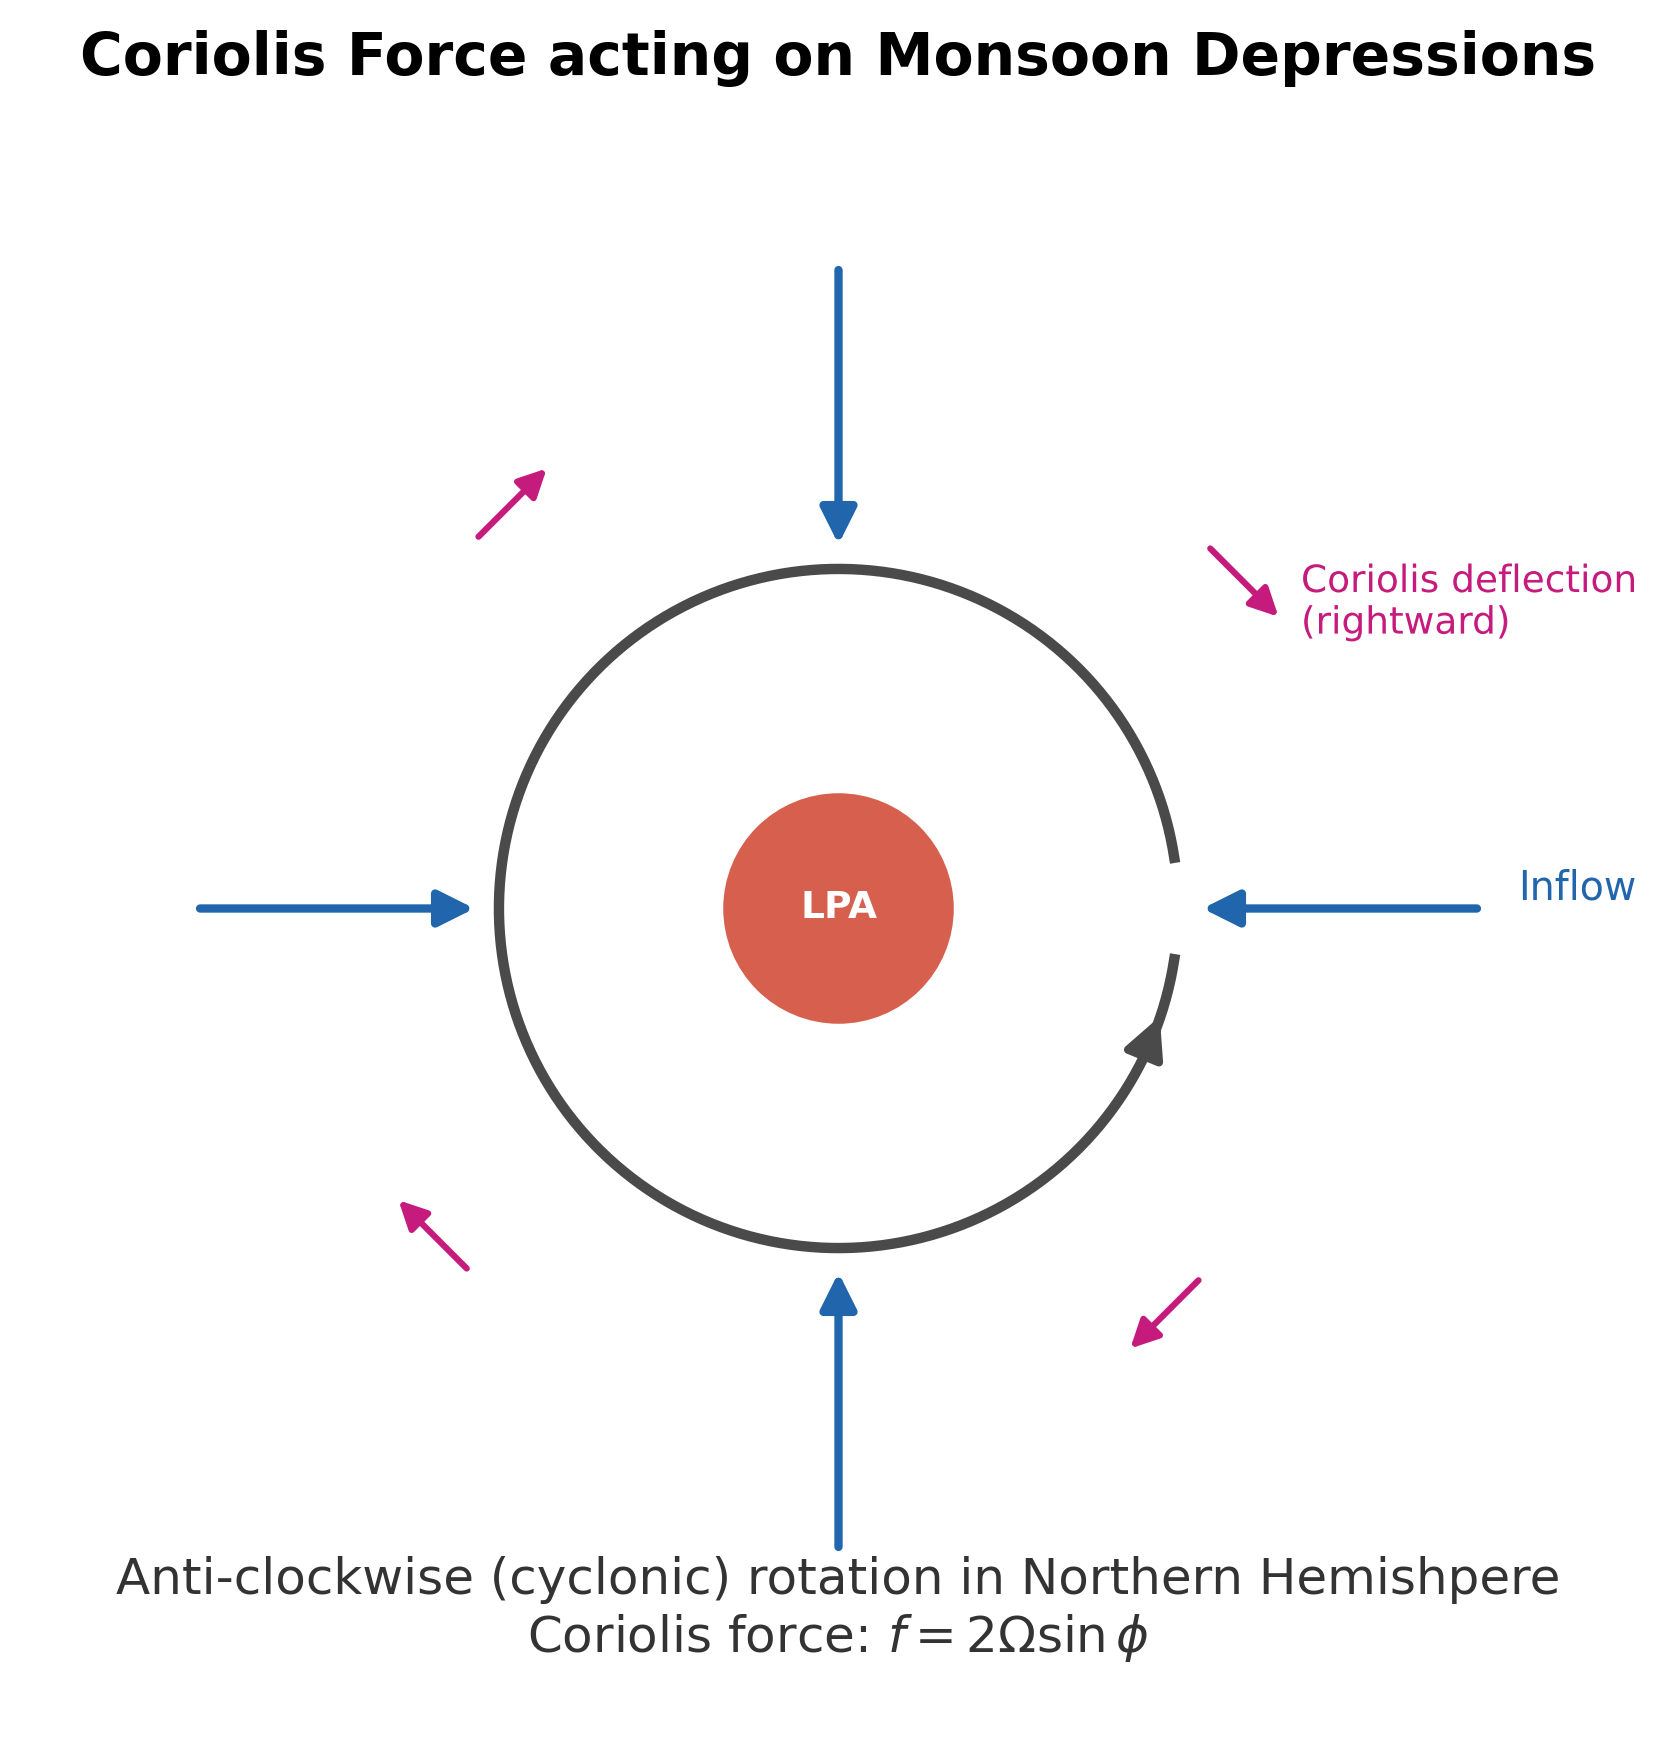
\includegraphics[width=0.60\textwidth]{Chapter2/Figs/coriolis_md_rotation.png}
  % \caption[Coriolis force and cyclonic rotation in the Northern
  % Hemisphere]{The
  %   Coriolis force deflects air parcels to the right in the
  % Northern Hemisphere.
  %   Air drawn toward a surface low (white arrows) is continuously deflected,
  %   producing anti-clockwise cyclonic rotation (curved arrows).}
  \caption[Coriolis force producing anti-clockwise MD
  rotation]{Boundary-layer air converging toward the MD center is
    deflected rightward by the Coriolis force, producing an
    anti-clockwise (cyclonic) circulation. The Coriolis parameter ($f =
  2\Omega\sin\phi$) increases with latitude.}%, setting the minimum
  % latitude ($\sim 5^\circ$N) for organised vortex development.}
  \label{fig:coriolis_bg}
\end{figure}

% \subsection{Why Monsoon Depressions Track North-Westward: The Role of
% Jet Streams}
% \label{subsec:md_nw_track}
%
% The characteristic north-westward translation of Indian MDs at
% 2-6\,m\,s$^{-1}$ results from two overlapping large-scale
% atmospheric controls, both of which are unique to the active Indian
% summer monsoon period.
%
% \subsubsection{The Monsoon Mean Flow and Trough Steering}
%
% An MD embedded in the lower troposphere is advected by the
% depth-averaged environmental wind in the 500-700\,hPa steering layer.
% During June-September, the large-scale monsoon circulation drives
% this steering flow broadly westward  and slightly poleward across the
% BoB and northern India. The \textbf{monsoon trough}, a semi-permanent
% axis of low pressure and enhanced cyclonic vorticity extending from
% the Pakistan-Rajasthan border, across Uttar Pradesh and Madhya
% Pradesh, to the BoB head-acts as the preferred corridor for LPS
% propagation, guiding systems north-westward along its axis
% \citep{sikka1977, mishra2021monsoon}. Systems forming at the BoB head
% are steered directly along this trough axis toward the
% Odisha-Gangetic plain coast.
%
% \subsubsection{The Somali Low-Level Jet and Sub-Tropical Westerly Jet}
% \label{subsubsec:jet_streams}
%
% Two jet systems exert decisive control on MD development and motion
% (Figure~\ref{fig:jet_streams_schematic}):
%
% \textbf{(1) The Somali Low-Level Jet (Findlater Jet):} This
% powerful south-westerly jet at 850-925\,hPa, first documented by
% \citet{findlater1969}, intensifies dramatically during the active
% ISM as the inter-hemispheric pressure gradient between the southern
% Indian Ocean and the heating Asian landmass maximises.
%
% The Findlater Jet channels large quantities of moisture-laden air
% from the Arabian Sea across the Indian peninsula into the BoB. In
% addition to its moisture supply role, the jet provides a powerful
% low-level steering current directed north-westward, which directly
% advects developing disturbances from the BoB head into the Indian
% interior. The jet core at 850\,hPa attains wind speeds of
% 20-30\,m\,s$^{-1}$ during active ISM spells and is the primary
% reason that MD tracks are so consistently directed toward Odisha,
% West Bengal, and Bihar rather than making arbitrary landfall along
% other coast segments.
%
% \textbf{(2) The Sub-Tropical Westerly Jet (STJ) and its poleward
% retreat:} During the pre-monsoon period (April-May), the STJ is
% positioned over northern India at approximately 200\,hPa, producing
% strong westerly vertical wind shear throughout the troposphere.
% This shear suppresses deep convective organisation and precludes MD
% development. As the monsoon onset occurs in June, the STJ abruptly
% jumps northward to a position at approximately 35-45$^\circ$N,
% entirely north of the Himalayas. With the STJ poleward of the
% Himalayan barrier, the upper-troposphere over the BoB and northern
% India becomes effectively \emph{decoupled} from the strong westerly
% shear. The resulting low-shear environment ($<10$\,m\,s$^{-1}$ over
% the BoB) is a necessary condition for MD deepening: a developing
% vortex is not ``sheared apart'' before it can organise
% \citep{holton2004introduction}. The monsoon onset therefore acts as
% a switch that simultaneously provides moisture (via the LLJ),
% reduces shear (via the STJ retreat), and establishes the monsoon
% trough axis along which MDs will propagate.
%
% % FIX: include better image
% \begin{figure}[H]
%   \centering
%   %% Note: DRAW THIS FIGURE - jet stream schematic
%   %% Elements to include:
%   %%   Thick blue arrow: Somali/Findlater Jet at 850 hPa (SW to NE
%   % across Indian Ocean + India)
%   %%   Thin red arrow: STJ poleward of Himalayan barrier at 200 hPa
%   %%   Cyclone symbol: over Bay of Bengal
%   %%   NW arrow: MD track direction
%   %%   Dashed line: monsoon trough axis across northern India
%   %%   Grey arc: Himalayan range
%   % \fbox{\rule{0pt}{5.5cm}\rule{0.75\textwidth}{0pt}}
%   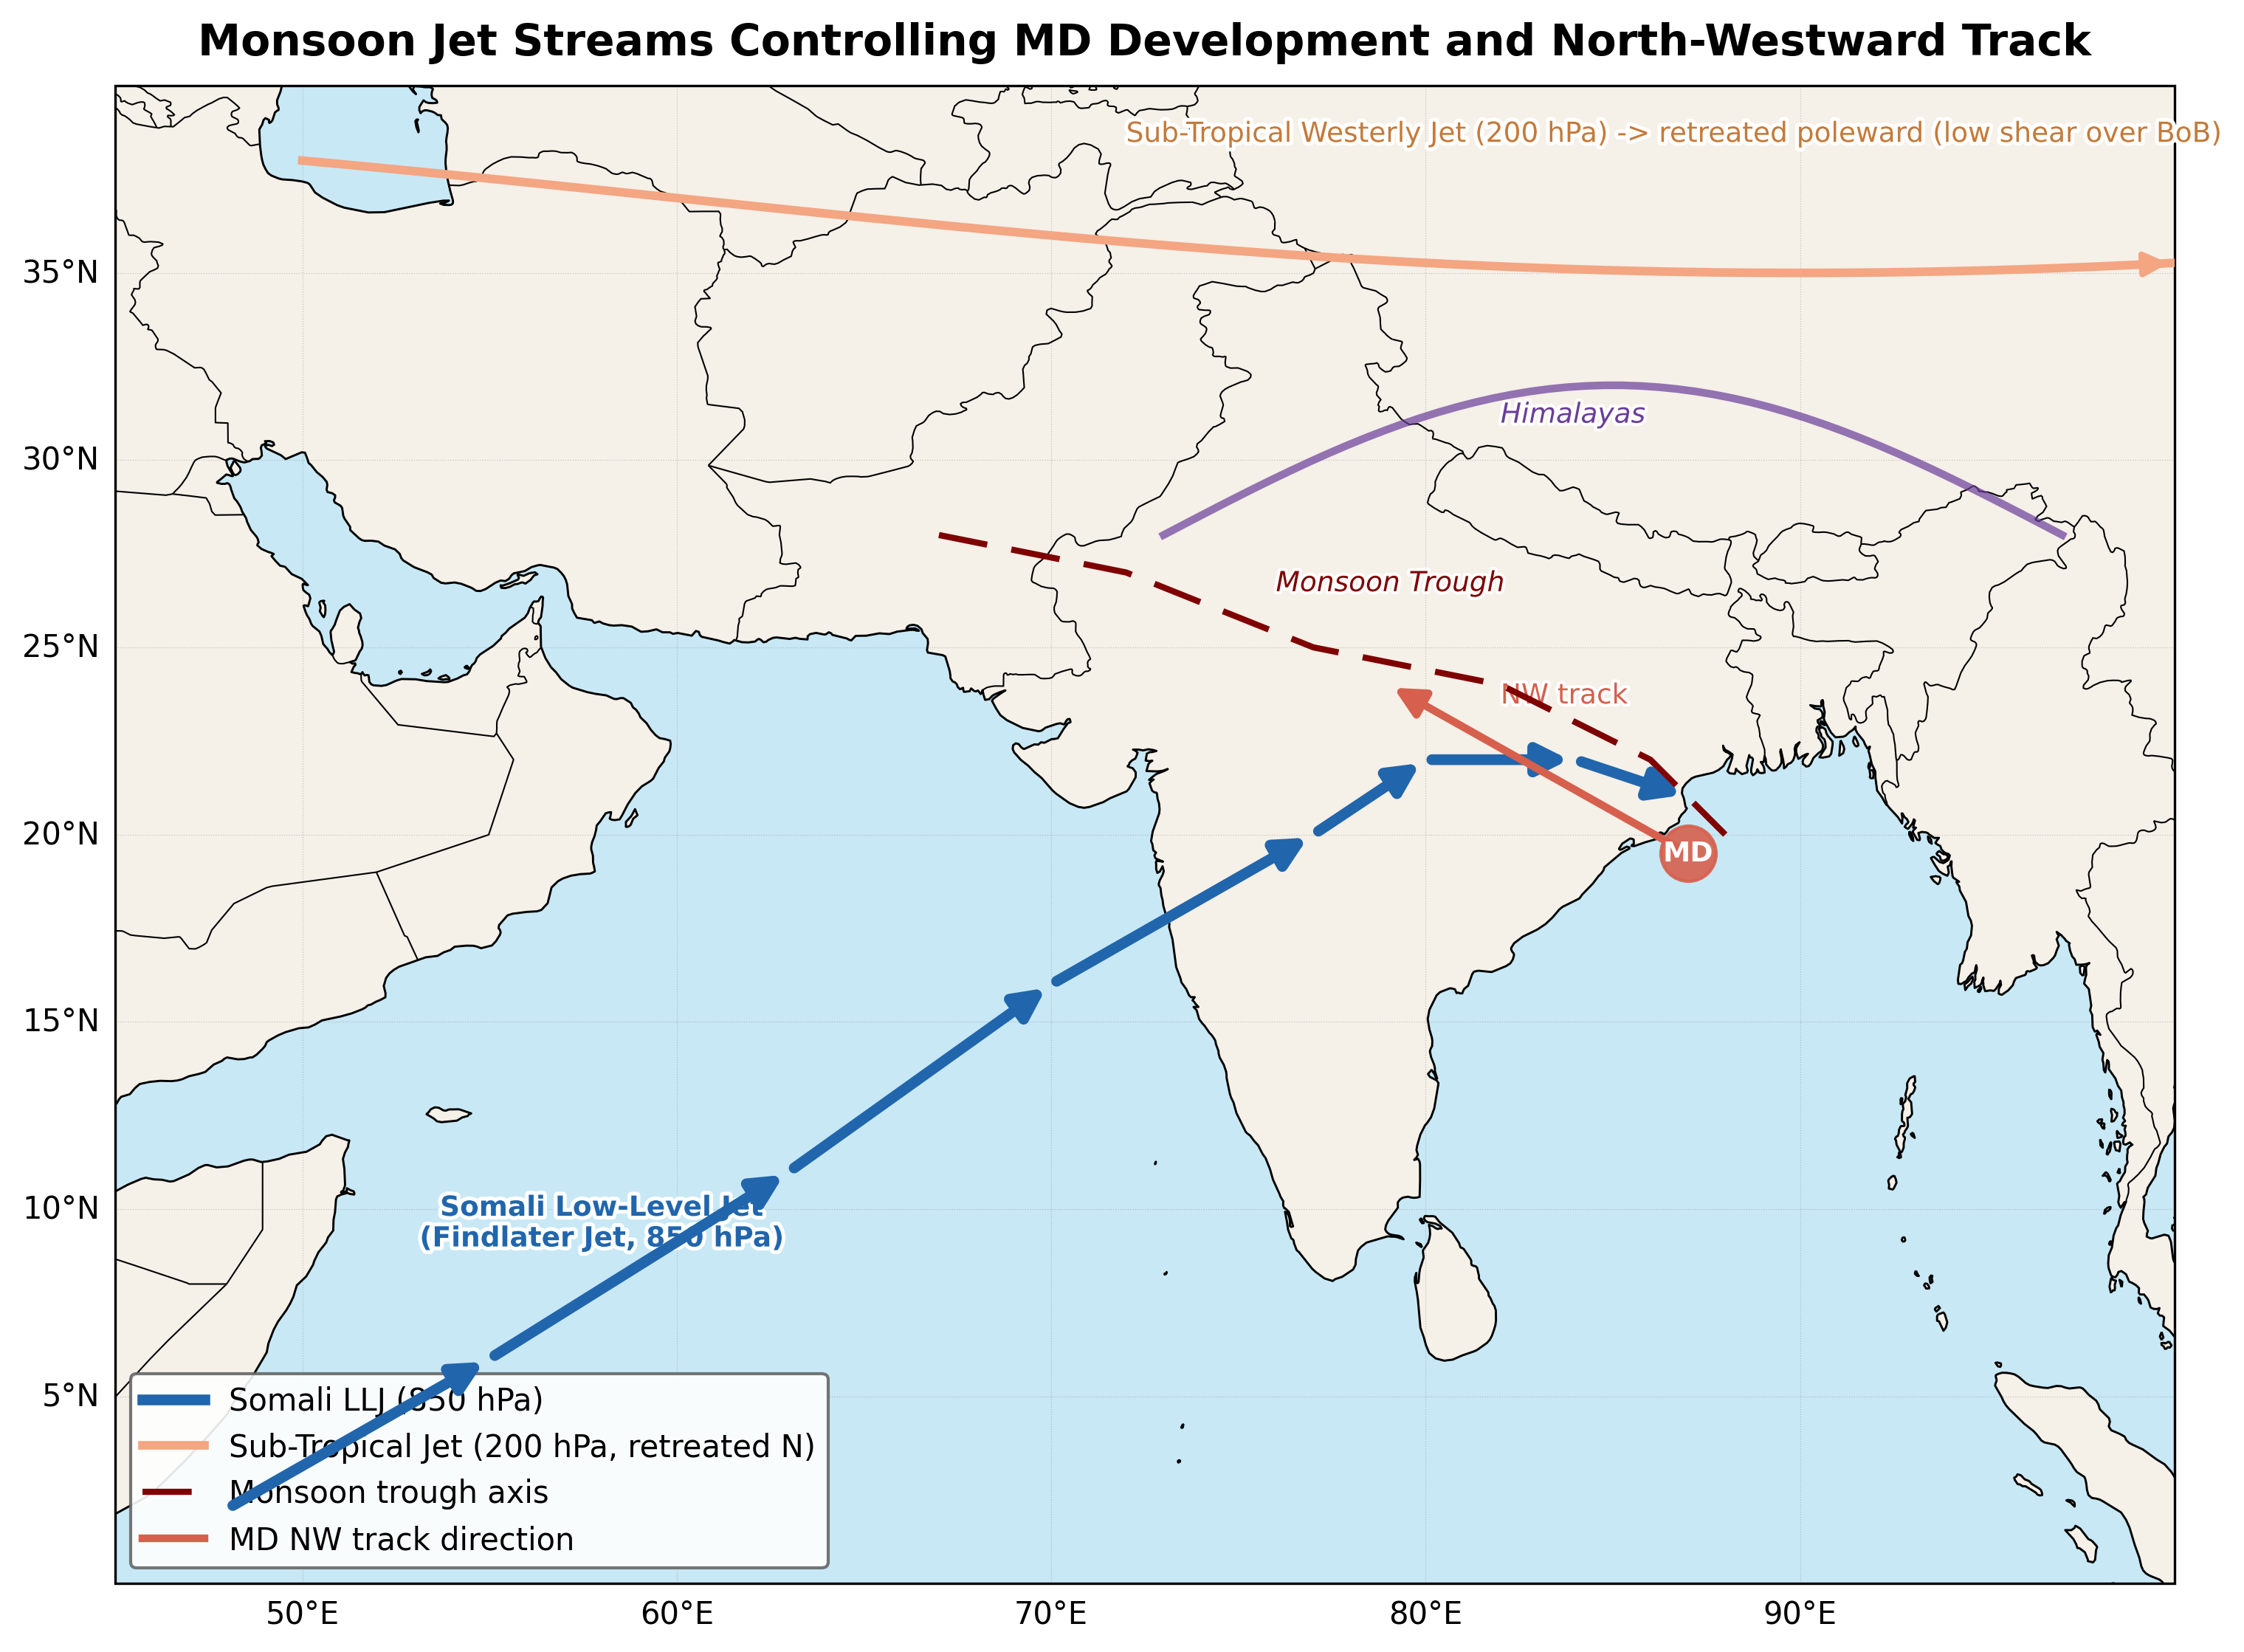
\includegraphics[width=0.75\textwidth]{Chapter1/Figs/jet_streams_schematic.png}
%   \caption[Monsoon jet streams controlling MD development and
%   north-westward motion]{Schematic showing the two jet systems
%     governing MD motion. The Somali Low-Level Jet (LLJ, thick arrow,
%     850\,hPa) supplies moisture and steers disturbances north-westward.
%     The Sub-Tropical Westerly Jet (STJ, thin arrow, 200\,hPa) has
%     retreated poleward of the Himalayas, eliminating destructive
%     upper-level wind shear over the BoB. The monsoon trough axis
%     (dashed) provides the preferred propagation corridor. After
%   \citet{findlater1969} and \citet{mishra2021monsoon}.}
%   \label{fig:jet_streams_schematic}
% \end{figure}

\subsection{Vortex Tilt: The Structural Integrity Diagnostic}
\label{subsec:vortex_tilt_background}

As an MD translates inland, the environmental vertical wind shear and
terrain-induced boundary-layer friction can cause the vortex to tilt:
the low-level (850\,hPa) center displaces relative to the upper-level
(200-300\,hPa) warm core.

\citet{rashid2005track} showed that a mature MD in the BoB typically
exhibits a small westward-northwestward tilt of 50-200\,km, the
direction dictated by the mean shear vector. This tilt is sustainable
so long as organised convection couples the upper and lower parts of
the vortex column through latent heat release.

After landfall, increased surface roughness decelerates the low-level
center faster than the upper-level flow, forcing the tilt to
increase. Once tilt exceeds a critical threshold, the
latent-heat-driven warm core decouples from the surface convergence
zone, convection weakens, and the vortex column rapidly loses
coherence-a structural precursor to terminal decay. The Brown Ocean
Effect counteracts this by sustaining boundary-layer convergence
(through continuous LHF) at the low-level center, keeping the
coupling alive even when the upper-level flow has advected the upper
warm core forward.

\section{The Brown Ocean Effect (BOE): Mechanism and Prior Literature}
\label{sec:boe_literature}

\subsection{Definition and Evidence}
\label{subsec:boe_original}

The BOE was formally introduced and named by \citet{andersen2013} in a global
climatological analysis of inland tropical cyclone maintenance events. They
identified numerous cases in which tropical systems over the continental United
States maintained or intensified over land and showed that these were associated
with sustained inland LHF meeting the criterion:
\begin{equation}
  \text{LHF}_{\text{inland}} \geq 70\;\text{W\,m}^{-2}
  \quad\text{for}\;\geq 18\;\text{consecutive hours post-landfall.}
  \label{eq:boe_def}
\end{equation}

% \yellownote{Add Tropical Storm Erin (2007) in reference and fix cite}
The canonical case study is Tropical Storm Erin (2007), which
unexpectedly re-intensified over Oklahoma to near-tropical-storm
intensity \citep{andersen2014insights}. Post-analysis revealed that
the Southern Great Plains had been saturated by heavy antecedent
rainfall, providing LHF at rates comparable to the Gulf of Mexico.

% \yellownote{Add Tropical Storm Bill (2015) in reference and fix cite}
\citet{wakefield2021} examined Tropical Storm Bill (2015) in detail
and provided the most complete documented case of the BOE feedback
loop, soil moisture near saturation at landfall maintained LHF
$>100$\,W\,m$^{-2}$, % which maintained CAPE,
which maintained organised precipitation that further wetted the
soil. The self-reinforcing character of this loop was identified as
the key mechanism enabling multi-day inland persistence.

\citet{nair2019influence} demonstrated the sensitivity of BOE
intensity to land cover type, urbanised and irrigated agricultural
surfaces enhanced the BOE signal relative to natural vegetation, a
finding relevant to the heavily irrigated Indo-Gangetic plains (IGP).

\subsection{BOE Evidence in the Indian Context}
\label{subsec:boe_india}

The translation of the BOE concept to Indian Monsoon Depressions is
recent and mostly model-based. \citet{kishtawal2013enhancement}
provided the first indirect observational evidence, using pre-storm
rainfall as a proxy for antecedent soil moisture, they demonstrated a
statistically significant positive relationship between the 15-day
pre-landfall cumulative rainfall along the future MD track corridor
and the subsequent inland penetration distance for 12 BoB depression
events. Their key finding were, heavier pre-storm rainfall (wetter
antecedent soil) produced longer inland persistence, is exactly what
the BOE predicts, but the mechanism (the LHF signal) was not directly
measurable from their proxy.

\citet{hunt2017effect} used a numerical weather prediction model to
systematically perturb the soil moisture initialisation for simulated
MDs. They found that higher soil moisture led to a warmer
mid-tropospheric core, enhanced precipitation, and longer inland life
cycles, confirming the mechanistic link between surface state and MD
post-landfall dynamics in a model framework.

\citet{osuri2020} demonstrated that assimilating satellite-derived
soil moisture (ASCAT) into the NWP initialisation significantly
improved simulated MD track and intensity, confirming the operational
relevance of the surface moisture state.

\citet{vijay2024boe} applied the BOE framework to the catastrophic
1999 Odisha Supercyclone, showing that antecedent soil moisture
pre-conditioned by a previous tropical system played a role in the
rapid intensification near and after landfall.

This study closes the gap between these proxy-based and modelling
approaches by directly measuring the LHF signal in ERA5 reanalysis
through the storm-centered Azimuthal Hovm\"{o}ller diagnostic.

% \section{Antecedent Soil Moisture: Pre-Conditioning and Soil Moisture Memory}
% \label{sec:soil_moisture_bg}
%
% \subsection{The Soil Moisture Evaporation Regime Transition}
% \label{subsec:sm_regime}
%
% The relationship between soil moisture and surface evaporation rate
% is non-linear and threshold-controlled
% \citep{seneviratne2010investigating}. Two regimes operate:
%
% \begin{enumerate}
%   \item \textbf{Water-limited regime} (dry soil, $\theta <
% \theta_\text{crit}$):
%     Evaporation is limited by the availability of soil water, not by
%     the available solar energy. LHF is proportional to $\theta /
%     \theta_\text{crit}$. In this regime, rainfall primarily
%     infiltrates into the soil (replenishing the deficit) rather than
%     evaporating immediately. Consequently, even heavy MD
%     precipitation may not raise LHF to BOE-sustaining levels if the
%     antecedent soil is very dry.
%   \item \textbf{Energy-limited regime} (wet soil, $\theta \geq
%     \theta_\text{crit}$): Soil is evaporating at its potential rate,
%     constrained only by the available net radiation, not by soil
%     water supply. LHF is at its maximum possible value for a given atmospheric
%     state, comparable to evaporation from an open water surface. This
%     is the regime in which the BOE operates. The critical threshold
%     $\theta_\text{crit}$ is approximately 65-75\,\% of the
%     soil's water holding capacity, corresponding to the matric
%     suction level at which hydraulic conductivity
%     begins to fall steeply \citep{clapp1978empirical}.
% \end{enumerate}
%
% For Gangetic clay loam-the dominant soil texture along the preferred
% MD track corridor over northern India-the Clapp-Hornberger exponent
% $\beta \approx 7.12$ \citep{clapp1978empirical}, implying that
% drainage slows dramatically as the soil approaches saturation and
% that near-saturated conditions ($\theta \geq \theta_\text{crit}$) are
% maintained for many days after heavy rainfall. This high soil
% moisture memory is precisely what enables multi-day BOE episodes:
% unlike sandy soils that drain and dry within hours, Gangetic clay
% loam retains near-capacity moisture for 3-7 days
% \citep{seneviratne2010investigating}.

\subsection{The Precipitation-Soil Moisture Positive Feedback}
\label{subsec:precip_sm_feedback}

The soil moisture feedback to precipitation-whereby wet soil produces
enhanced surface evaporation, which moistens and destabilises the
boundary layer, which intensifies convection and precipitation-is
observationally established over India at synoptic and intra-seasonal
timescales \citep{longterm2025, wei2016impact}.
The mechanism proceeds through two pathways:

\clearpage
\begin{enumerate}
  \item \textbf{Thermodynamic pathway:} Moist soil suppresses daytime
    sensible heating (lowering Bowen ratio$\beta$), reducing the height of the
    convective boundary layer and increasing near-surface specific humidity $q$.
    This raises the equivalent potential temperature ($\theta_e$)
    \citep{bolton1980computation} at the surface, increasing CAPE and
    convective triggering probability.
    \begin{equation}
      \theta_e = T_K(P_0/P)^{R_d/c_p}\exp(L_v q / c_p T_L)
    \end{equation}
    where:\\
    $T_K$ is the absolute temperature at pressure $P$, \\
    $P_0$ is the reference pressure (usually 1000 hPa), \\
    $R_d$ is the gas constant for dry air, \\
    $c_p$ is the specific heat of dry air at constant pressure, \\
    $L_v$ is the latent heat of vaporization, \\
    $q$ is the specific humidity, \\
    $T_L$ is the temperature at the lifting condensation level.
  \item \textbf{Dynamic pathway:} Enhanced LHF at the land surface
    increases the low-level moisture flux convergence into the MD
    vortex-a process directly analogous to the oceanic surface flux
    maintaining the vortex over the BoB.
    % The key observational test implemented in this study, is the
    % Granger causality of total precipitation on subsequent SWVL1: if
    % precipitation significantly Granger-causes soil moisture (with
    % the expected positive sign), the active self-wetting component of
    % the BOE is confirmed in the ERA5 record.
    % \yellownote{TODO: Granger tests}
\end{enumerate}

% \subsection{The ASMI as a Pre-Landfall Predictor}
% \label{subsec:asmi_background}
%
% Building on \citet{kishtawal2013enhancement}, this study employs an
% \emph{exponentially weighted} Antecedent Soil Moisture Index (ASMI)
% that (i) uses direct ERA5 \texttt{SWVL1} measurements rather than
% precipitation proxies, (ii) weights recent soil moisture more heavily
% than older conditions ($\kappa^d$, $\kappa = 0.85$), and (iii)
% computes the index specifically over the \emph{future inland track
% corridor} rather than the current position.
%
% The 7-day lag is theoretically motivated: it corresponds to the
% dominant soil moisture memory timescale of Gangetic clay loam (3-7
% days), meaning that the soil moisture 7 days before landfall best
% represents the background wetness state rather than being
% contaminated by either the MD's own recent rainfall or ephemeral dry spells.

\section{The Eastern Ghats: Orographic Barrier and Research Finding}
\label{sec:eastern_ghats_bg}

\subsection{Physical Geography and Structure}
\label{subsec:ghats_geography}

The Eastern Ghats are a discontinuous range of hills running
approximately north-northeast to south-southwest along the eastern
margin of the Deccan Plateau, at a general inland distance of
100-300\,km from the Bay of Bengal coast (Figure~\ref{fig:eastern_ghats_map}).

\begin{figure}[H]
  \centering
  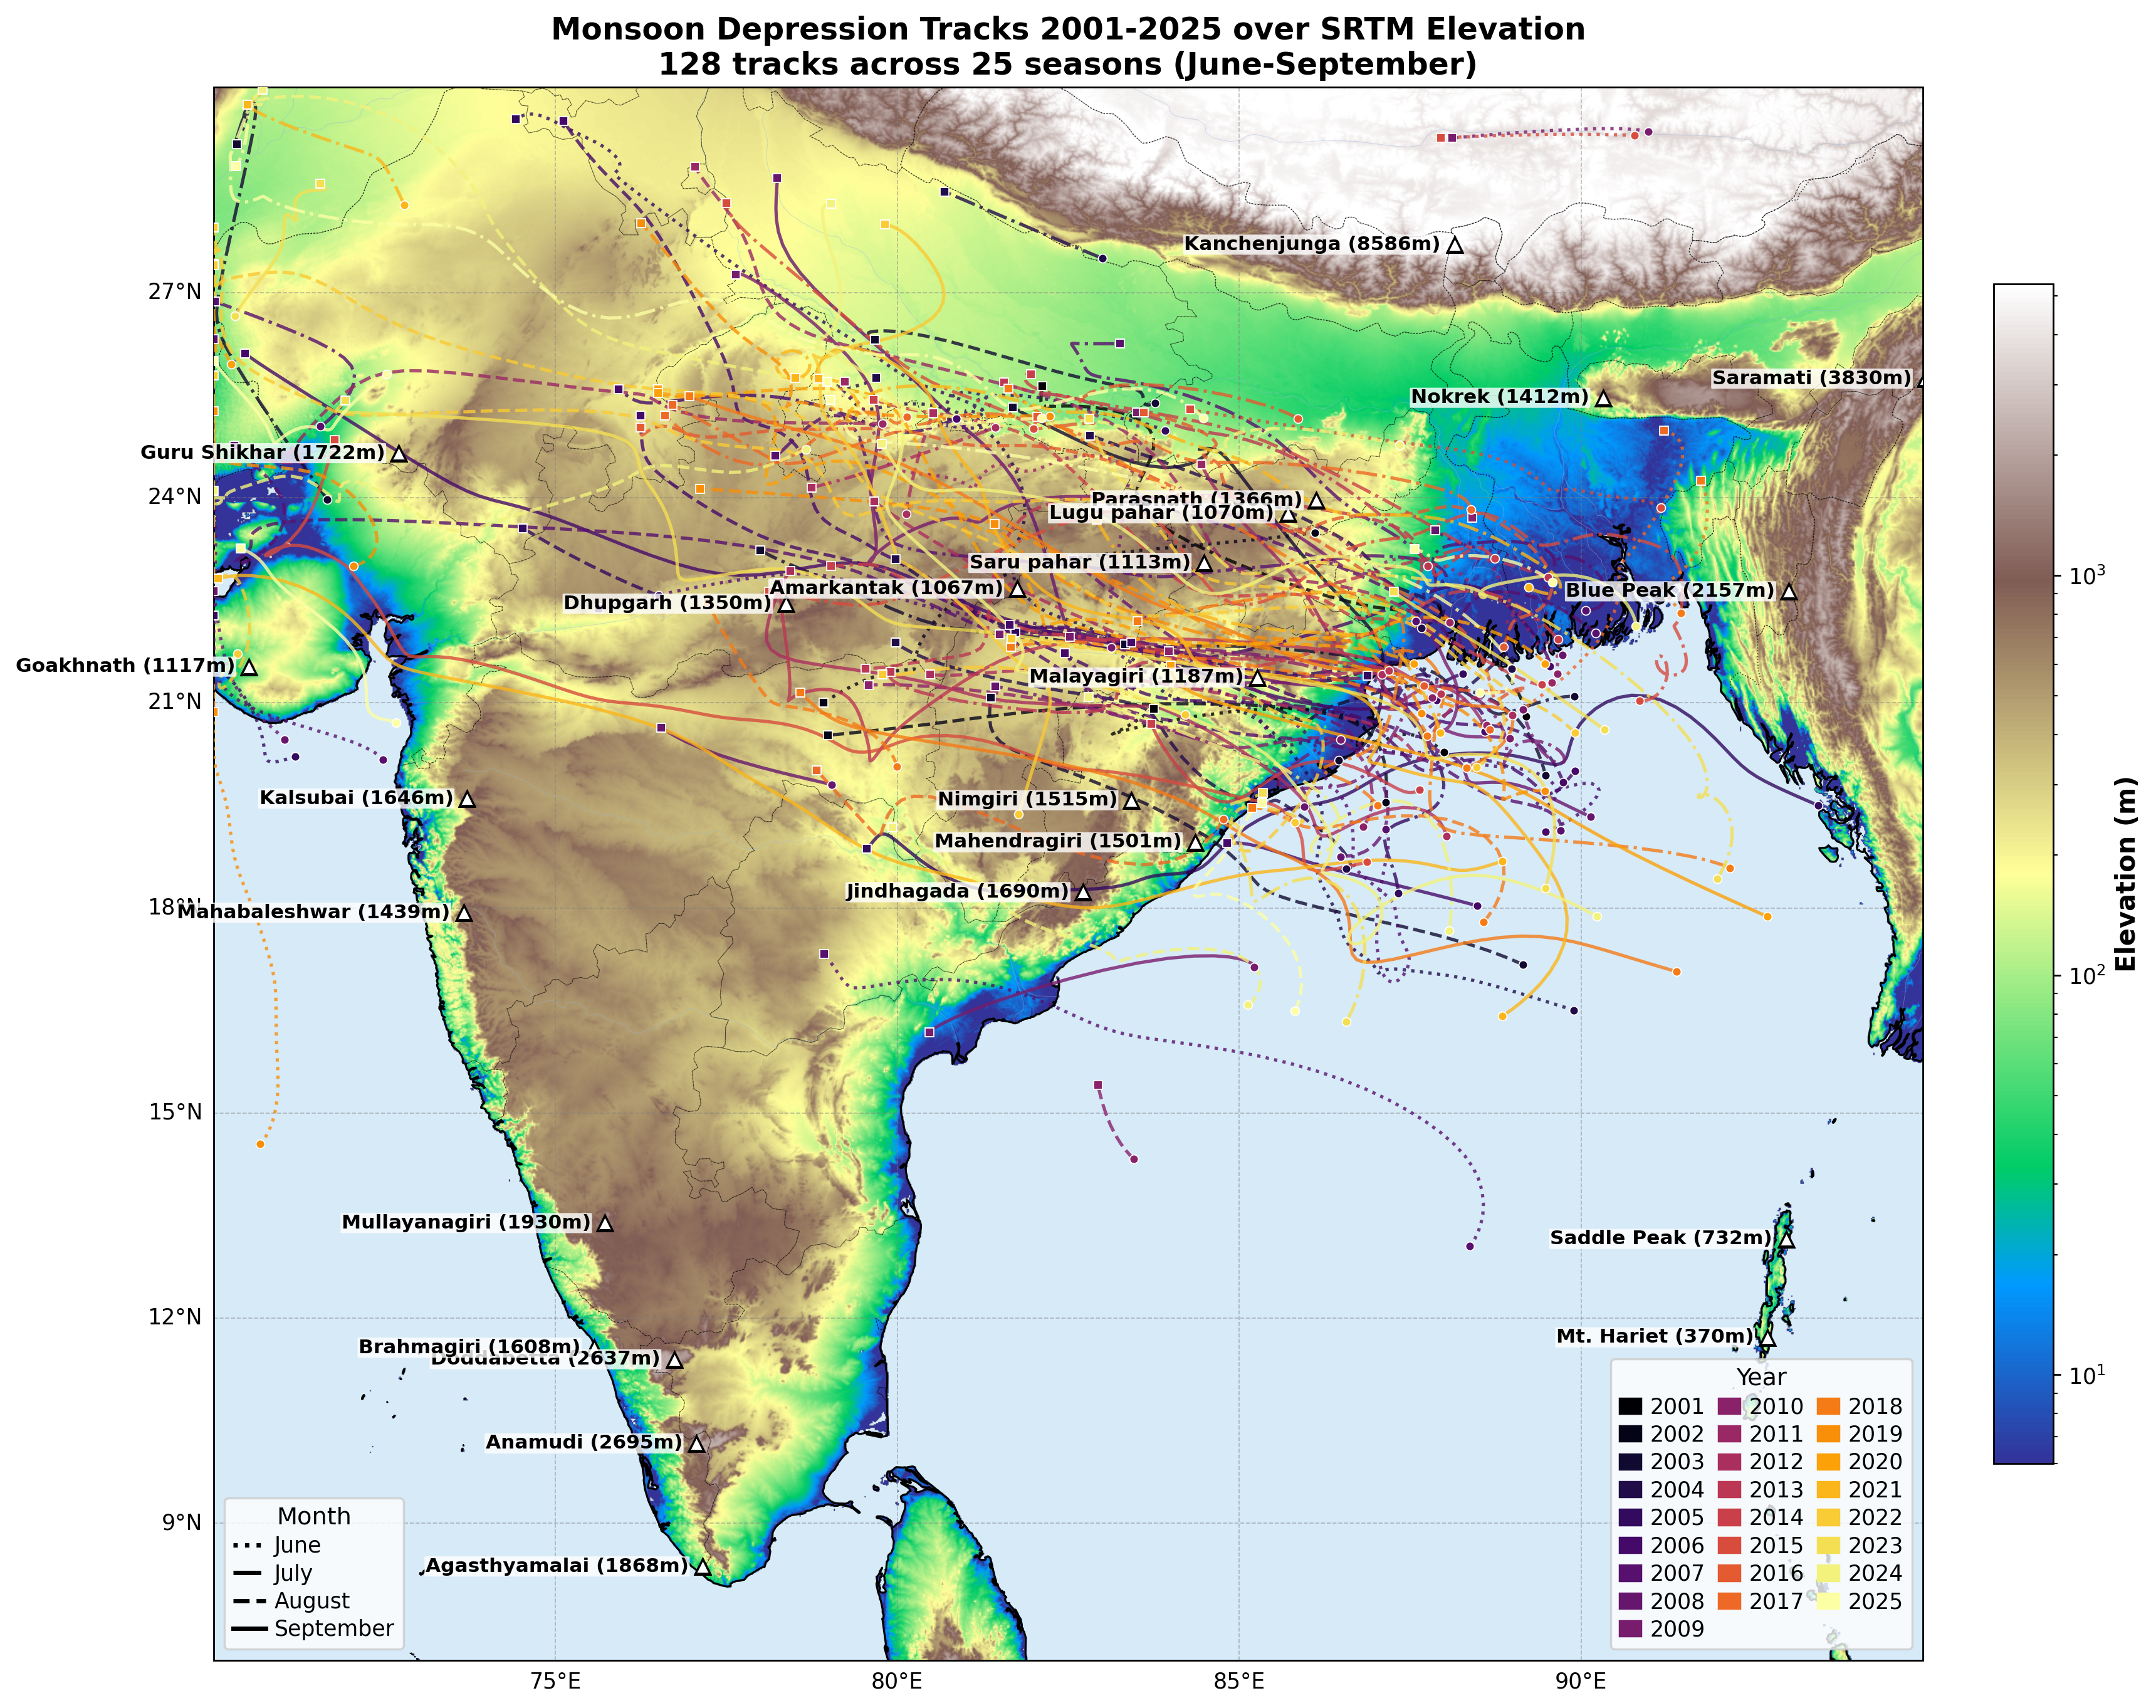
\includegraphics[width=0.76\textwidth]{Chapter2/Figs/all_years_tracks_elevation.png}
  \caption[Terrain elevation map of the Eastern Ghats and MD landfall
  zone]{All MD tracks from ERA5 (2001-2025). Colours and line style
    represents duration (year and months respectively) and contours
    represents elevation from SRTM. SRTM digital elevation model (m) of
  the Eastern Ghats and the eastern Deccan Plateau.}
  % The discontinuous ridge at 600-1000\,m is interrupted by the
  % Mahanadi (north), Godavari (south), and Brahmani river-valley gaps.
  % MD landfall tracks typically traverse the range within 24-48
  % hours of crossing the coast.}
  \label{fig:eastern_ghats_map}
\end{figure}
\vspace{-0.7cm}
\begin{figure}[H]
  \centering
  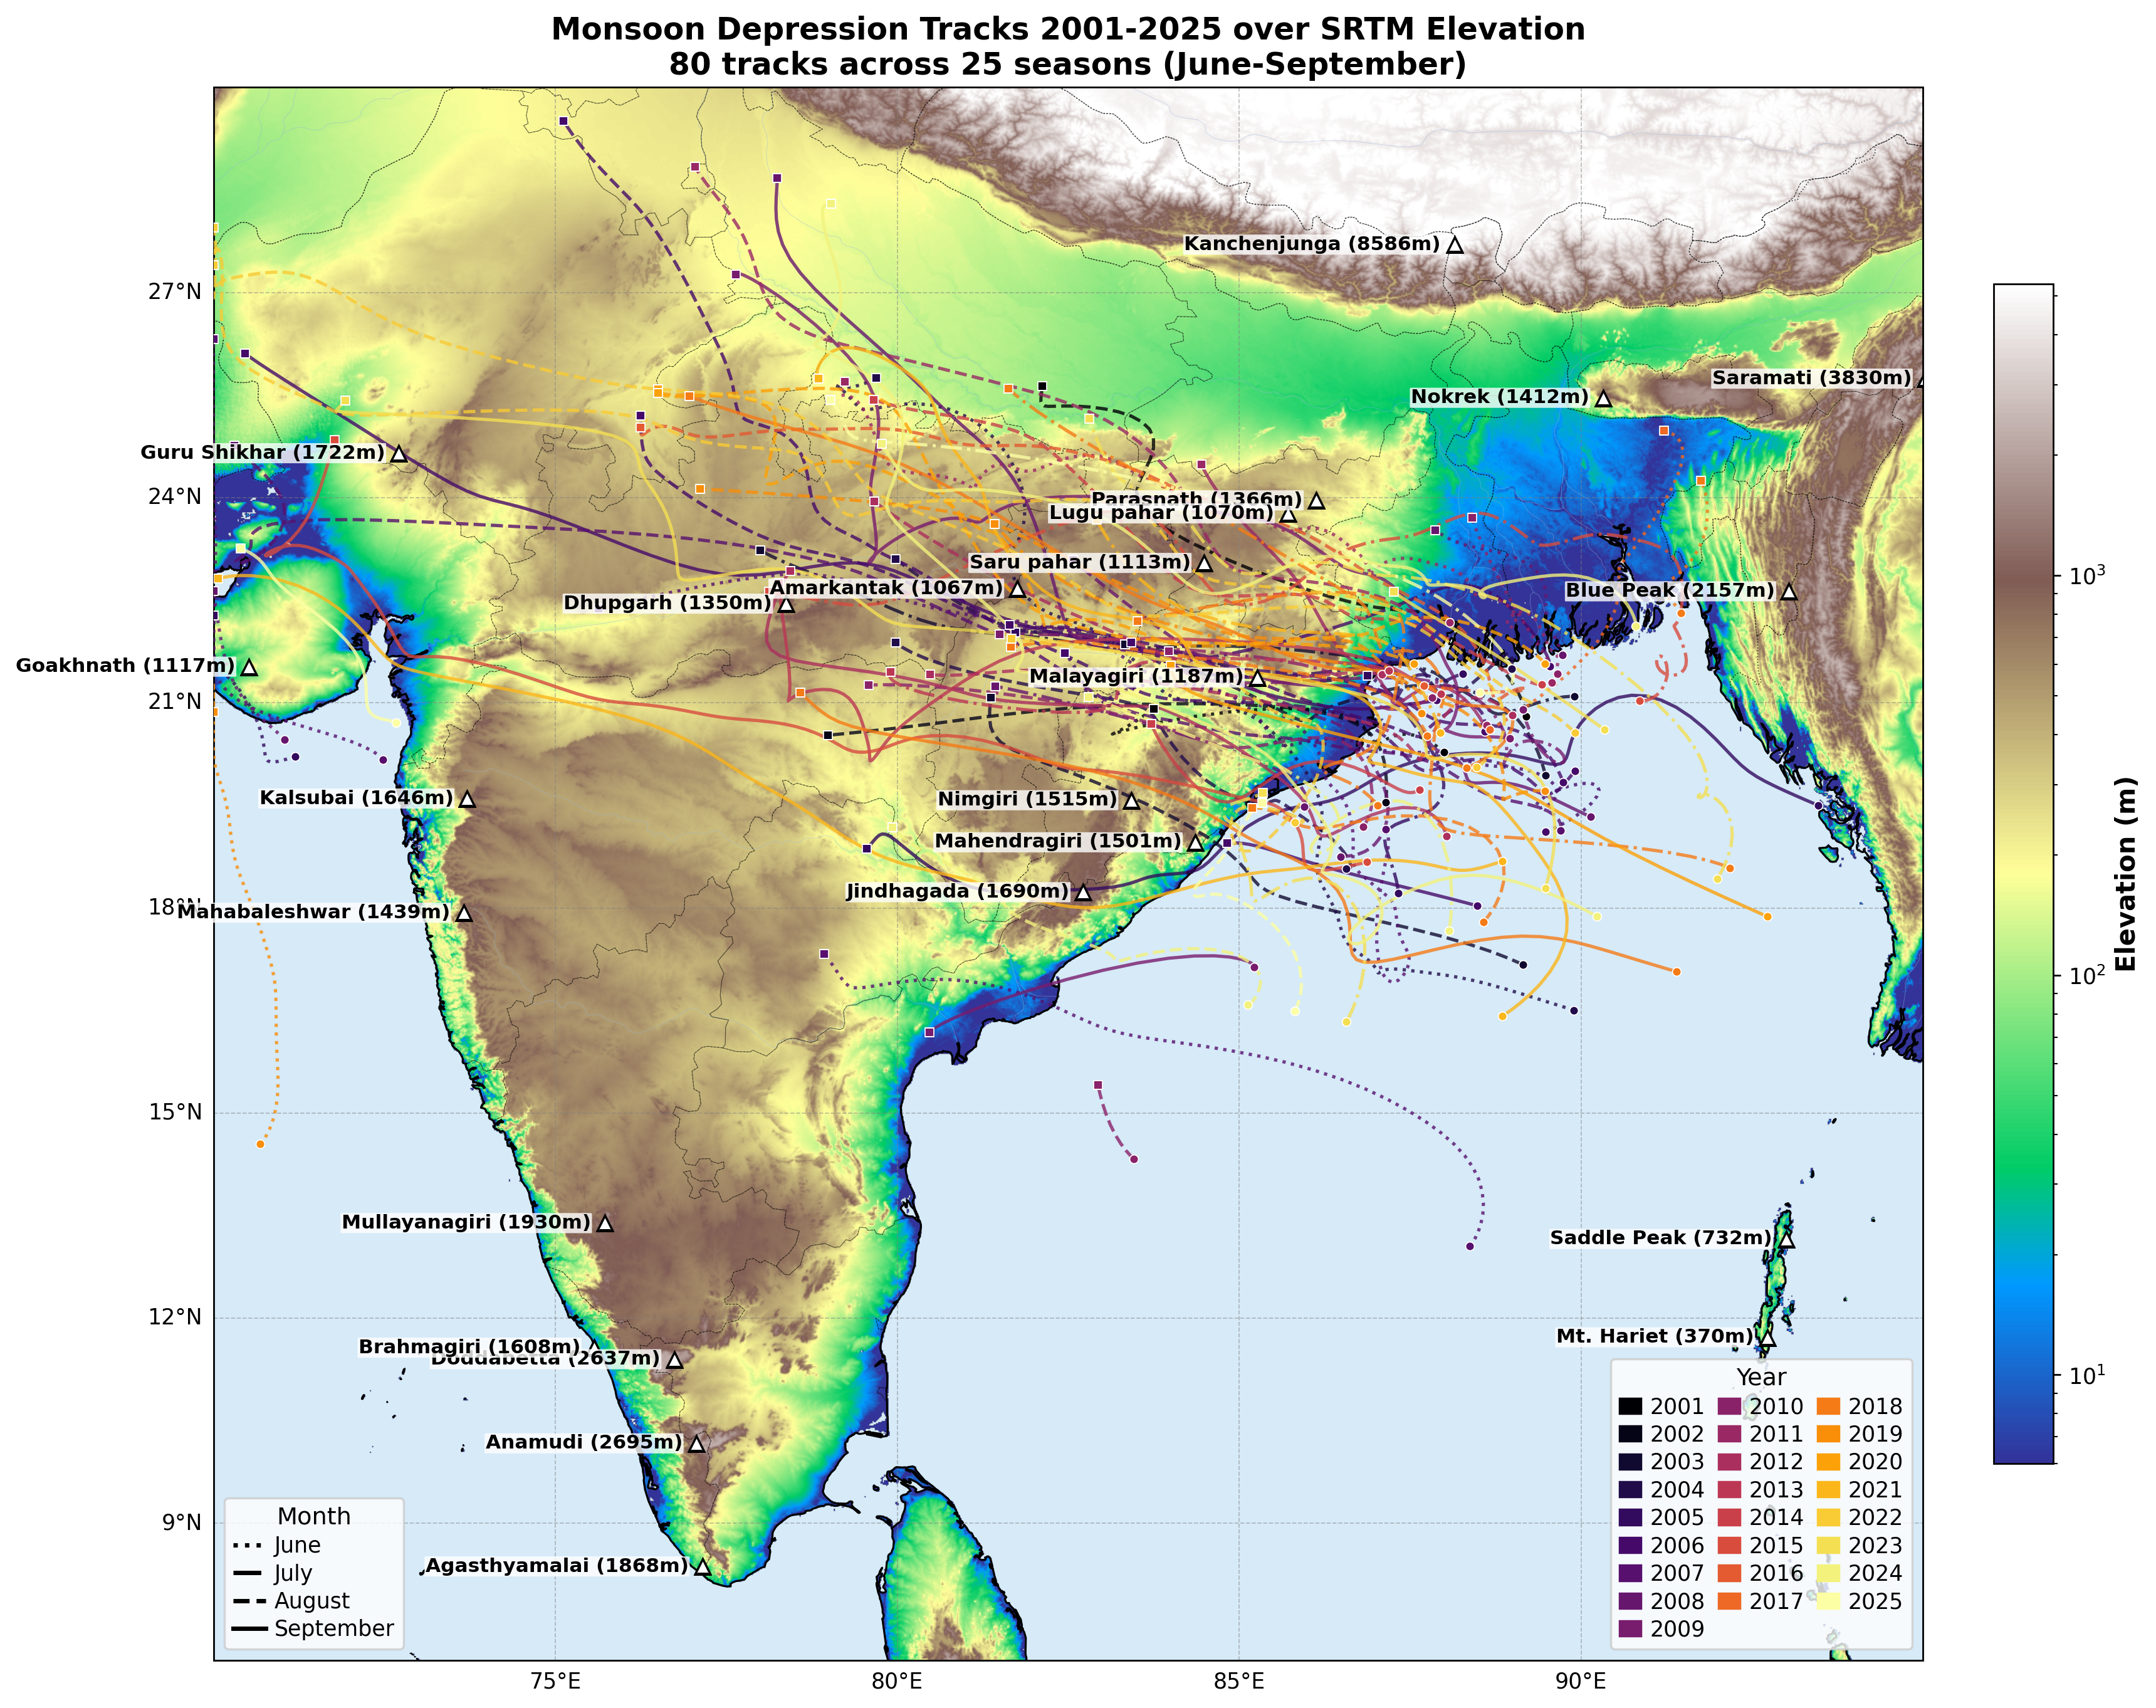
\includegraphics[width=0.75\textwidth]{Chapter1/Figs/ocean_only_tracks.png}
  \caption[Monsoon Depression track climatology of Ocean
  organinateMDs, 2001-2025]{Ocean organised MD tracks from ERA5
    (2001-2025). Colours and line style represents duration (year and
  months respectively) and contours represents elevation from SRTM.}
  \label{fig:ocean_md_tracks}
\end{figure}

Unlike the continuous, high-elevation Western Ghats (2000-2500\,m),
the Eastern Ghats are fragmented by major river systems-the Mahanadi,
Godavari, and Brahmani rivers cross the range through wide
river-valley gaps-with typical average elevations of 600-1000\,m
(with highest peaks reaches around 1600\,m). The overall range width
is approximately 80-200\,km, and the mean slope angle of the windward
(eastern) face is shallow (1-3$^\circ$), making the Ghats moderate
rather than catastrophic orographic barrier. This geographic
structure has a critical implication for MD dynamics: the Ghats are
wide enough and high enough to impose significant orographic forcing,
yet gaps are wide enough to sometimes allow MD's low-level
circulation to partially pass through without the full brunt of
barrier blocking-making the \emph{landfall longitude} relative to gap
positions a potentially important predictor of inland penetration.

\subsection{Four Mechanisms by Which the Eastern Ghats Block or Weaken MDs}
\label{subsec:ghats_mechanisms}

When an MD crosses the Eastern Ghats, four simultaneous physical
processes engage.
Together, these constitute the orographic modulation mechanism that
this thesis identifies as a major determinant of post-landfall fate:

\begin{enumerate}
  \item \textbf{Mechanism 1: Orographic precipitation enhancement and
    moisture removal.} Forced ascent on the windward (eastern)
    face of the Ghats  triggers orographic convection, substantially
    enhancing precipitation rates on the eastern slopes
    \citep{houze1994, orographyconvection2005, medina2003analysis}.
    For a saturated, convectively unstable air column such as that
    within an MD, even modest forced ascent of 10-20\,cm\,s$^{-1}$
    over the 600-1000\,m terrain can release latent heat equivalent
    to deep convection. While this enhancement temporarily
    intensifies the MD's apparent rainfall on its eastern flank, it
    is simultaneously removing moisture from the inflowing
    boundary-layer air before it reaches the inner vortex. The result
    is that the MD's moisture budget is \emph{depleted} faster on the
    windward side than over the flat coastline, reducing the moisture
    available to sustain inner-core convection on the leeward side.
  \item \textbf{Mechanism 2: Translational speed deceleration.} As
    the MD crosses the terrain, increased surface roughness and the
    mechanical blocking effect of the elevated range decelerate the
    system's forward motion.
    % This deceleration is quantified in this study through the
    % Terrain Sensitivity Index (TSI).
    The deceleration has two consequences: (i) the MD spends more
    time over the windward slope, leading to extreme localised
    rainfall enhancement on the eastern Ghats face; and (ii) the
    low-level center stalls relative to the upper-level flow, forcing
    an increase in vortex tilt (Mechanism 4).
    % In some cases, MDs can become quasi-stationary over the Ghats for
    % hours before either crossing or dissipating. The degree of
    % blocking can be quantified through the \emph{Froude number}
    % approach \citep{houze1994}:
    % \begin{equation}
    %   Fr = \frac{U}{Nh},
    %   \label{eq:froude}
    % \end{equation}
    % where $U$ is the approaching flow speed (MD translation speed,
    % $\approx 3$-5\,m\,s$^{-1}$), $N$ is the Brunt-Vaisala frequency
    % of the impinging air column, and $h$ is the terrain height
    % (600-1000\,m for the Eastern Ghats). When $Fr < 1$, the flow
    % tends to deflect around the barrier (blocking regime); when $Fr >
    % 1$, it can flow over the terrain. For typical MD conditions ($N
    % \approx 0.01$\,s$^{-1}$, $h = 800$\,m), $Fr \approx 0.4$-0.6,
    % placing MDs squarely in the partially-blocked regime, consistent
    % with observed speed reduction but not complete stoppage.
  \item \textbf{Mechanism 3: Low-level easterly moisture inflow
    blocking.} The most consequential effect of the Eastern Ghats on
    MD energetics is the blockage of the low-level easterly moisture
    inflow from the BoB. Pre-landfall, the MD draws a continuous
    supply of warm, moisture-laden air from the Bay of Bengal through
    its eastern sector (the inflow region), sustaining the water
    vapour mixing ratio in the inner core. As the terrain obstructs
    this inflow, the Integrated Vapour Transport (IVT) from the BoB
    peaks around at 300K drops sharply (Figure~\ref{fig:ivt_example}).
    On the leeward side, the MD must draw on local surface
    evapotranspiration (if BOE-active) or face rapidly declining
    moisture availability in its inner core.
    The transition from \emph{oceanic} moisture inflow to \emph{local
    surface} moisture supply at the terrain crossing is the fundamental
    energy-source switch this thesis documents.
  \item \textbf{Mechanism 4: Vortex Tilt and Structural Decoupling.}
    The Eastern Ghats selectively slow the low-level (850\,hPa) MD
    center while the upper-level (200-300\,hPa) anticyclonic outflow,
    being largely unaffected by surface terrain, continues to
    propagate westward at the large-scale steering speed. The result
    is an increasing westward displacement of the upper warm core
    relative to the low-level vortex-an increasing vortex tilt
    (Section~\ref{subsec:vortex_tilt_background}). When the tilt
    exceeds the critical threshold, the latent heat release in the
    convective updrafts no longer efficiently maintains the warm core
    above the surface convergence zone, and the vortex loses vertical
    coherence. This is the structural mechanism of terrain-induced
    weakening. The Vortex Tilt analysis directly measures this
    evolution (Figure~\ref{fig:vortext_tilt}).
\end{enumerate}

% \begin{figure}[H]
%   \centering
%   %% Note: DRAW THIS FIGURE - cross-section schematic showing:
%   %%   Left (east): BoB, MD circulation, easterly moisture inflow arrows
%   %%   center: Eastern Ghats (600-1000m hill profile)
%   %%   Windward side: forced ascent, orographic rain enhancement (raindrops)
%   %%   Leeward side: descending dry air (foehn), vortex tilt arrow
%   %%   Upper arrows: upper-level flow continuing westward faster
% than low-level
%   %%   Label: "Low-level center stalls", "Upper warm core advances",
%   % "IVT blocked"
%   \fbox{\rule{0pt}{7cm}\rule{0.90\textwidth}{0pt}}
%   % \includegraphics[width=0.90\textwidth]{Chapter2/Figs/ghats_blocking_schematic}
%   \caption[Schematic of Eastern Ghats orographic modulation of a
%   landfalling MD]{East-west cross-section showing the four mechanisms
%     by which the Eastern Ghats modulate a landfalling MD. (1)
%     Orographic precipitation enhancement on the windward face depletes
%     the moisture column. (2) Frictional deceleration stalls the
%     low-level center. (3) Low-level easterly BoB moisture inflow is
%     blocked by the terrain. (4) The upper-level warm core continues
%     westward faster than the surface low, increasing vortex tilt.
%     BOE-candidate systems counteract mechanisms 3 and 4 through
%   sustained surface LHF on the leeward side.}
%   \label{fig:ghats_blocking_schematic}
% \end{figure}
\begin{figure}[H]
  \centering
  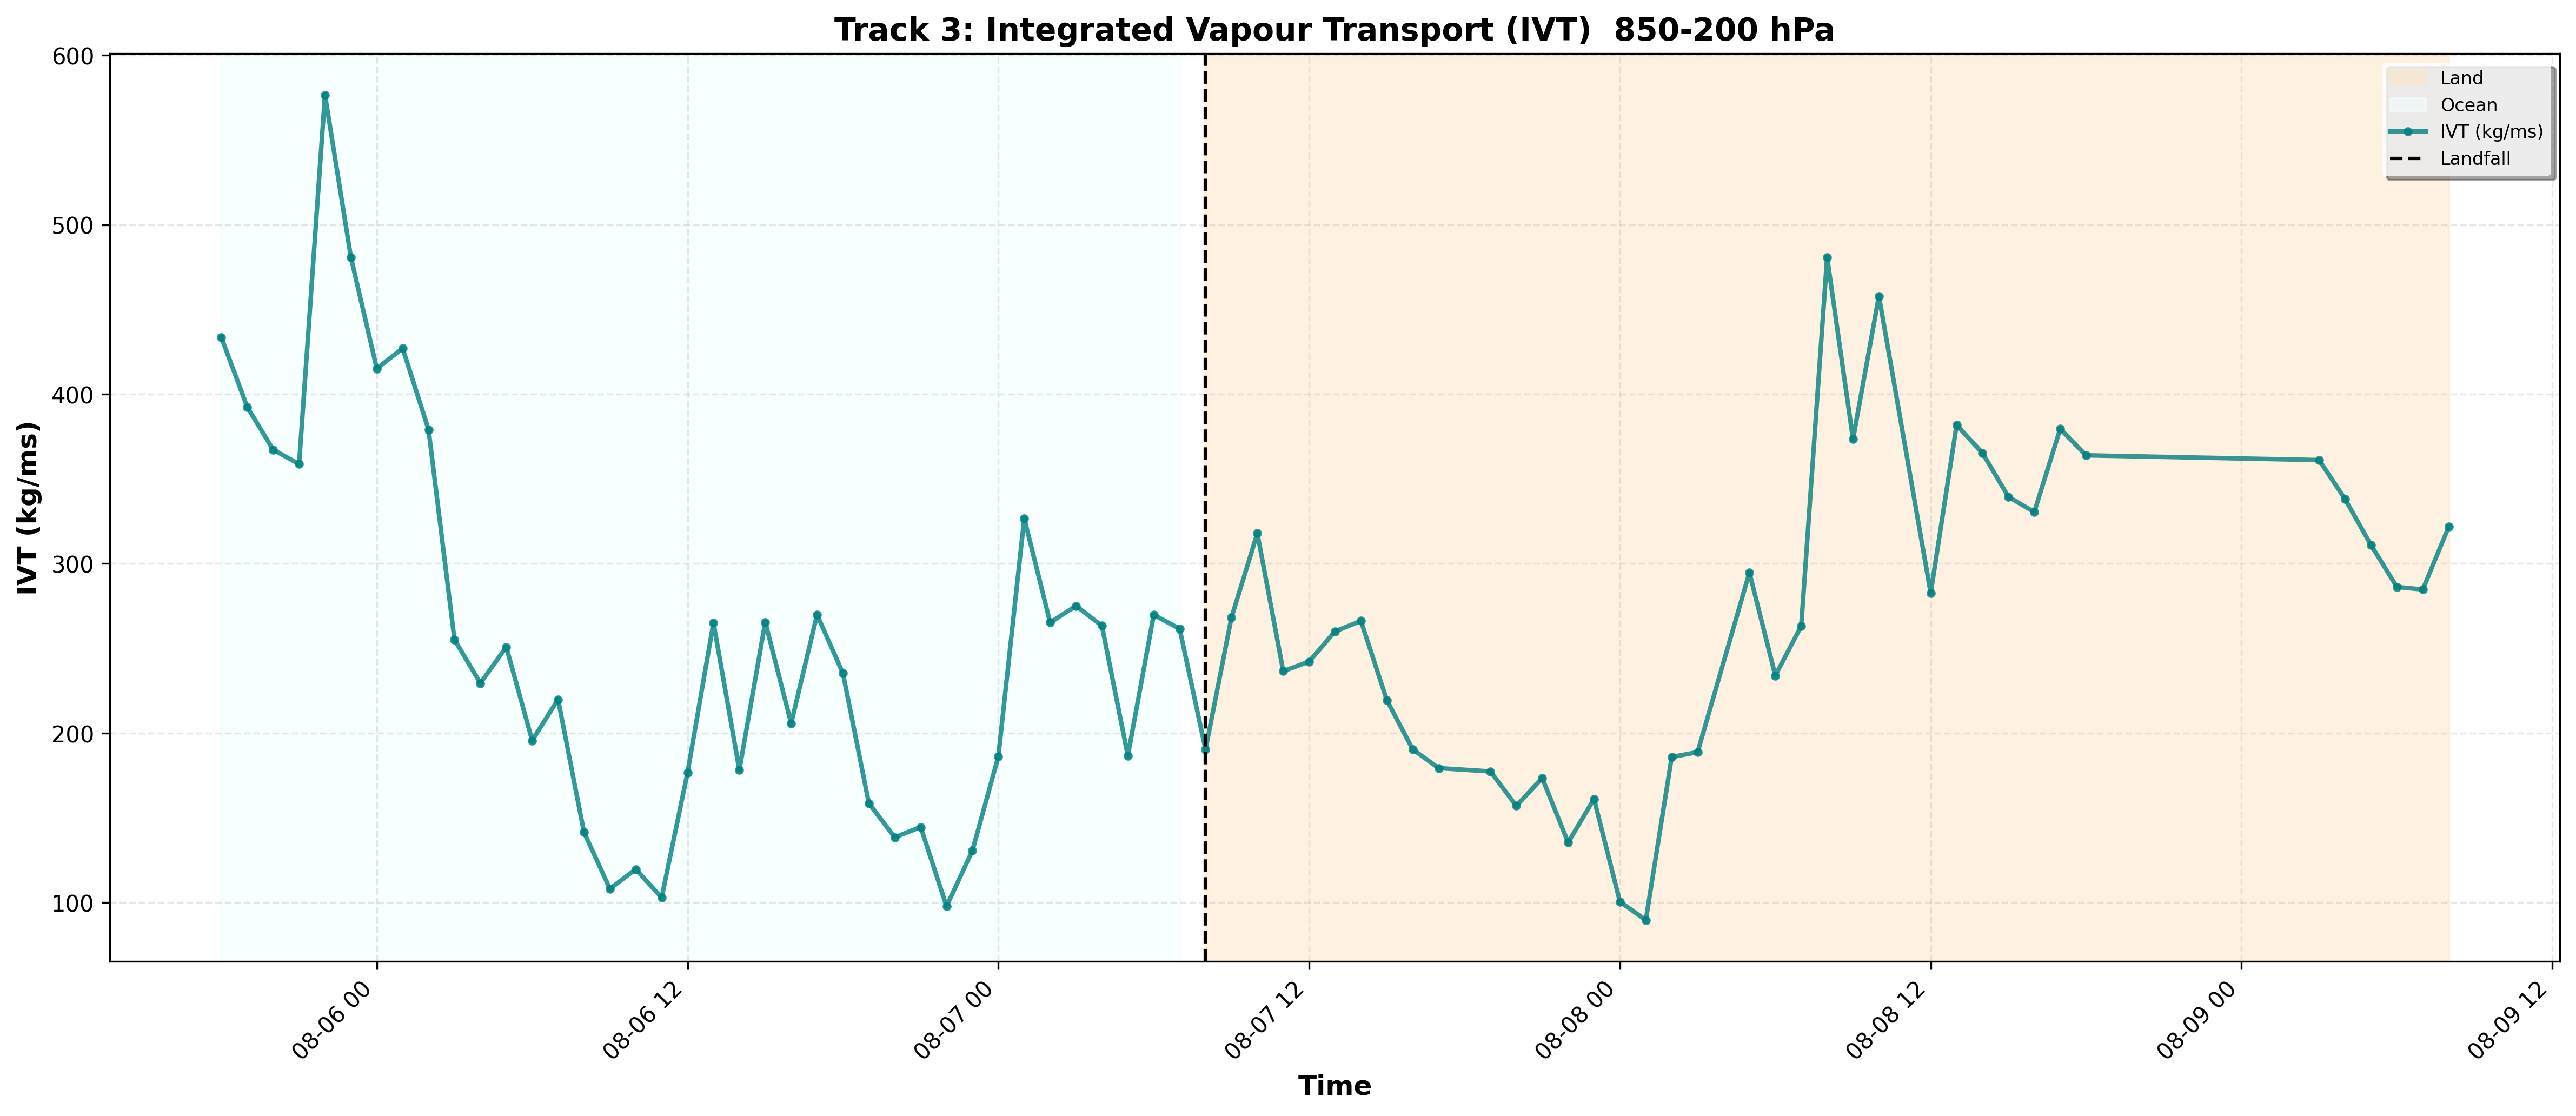
\includegraphics[width=0.95\textwidth]{Chapter2/Figs/ivt_example}
  \caption{Integrated Vapour Transport (IVT) analysis showing the
    sharp increase then drop in moisture flux from the Bay of Bengal as the MD
  encounters land.}
  \label{fig:ivt_example}
\end{figure}

\begin{figure}[H]
  \centering
  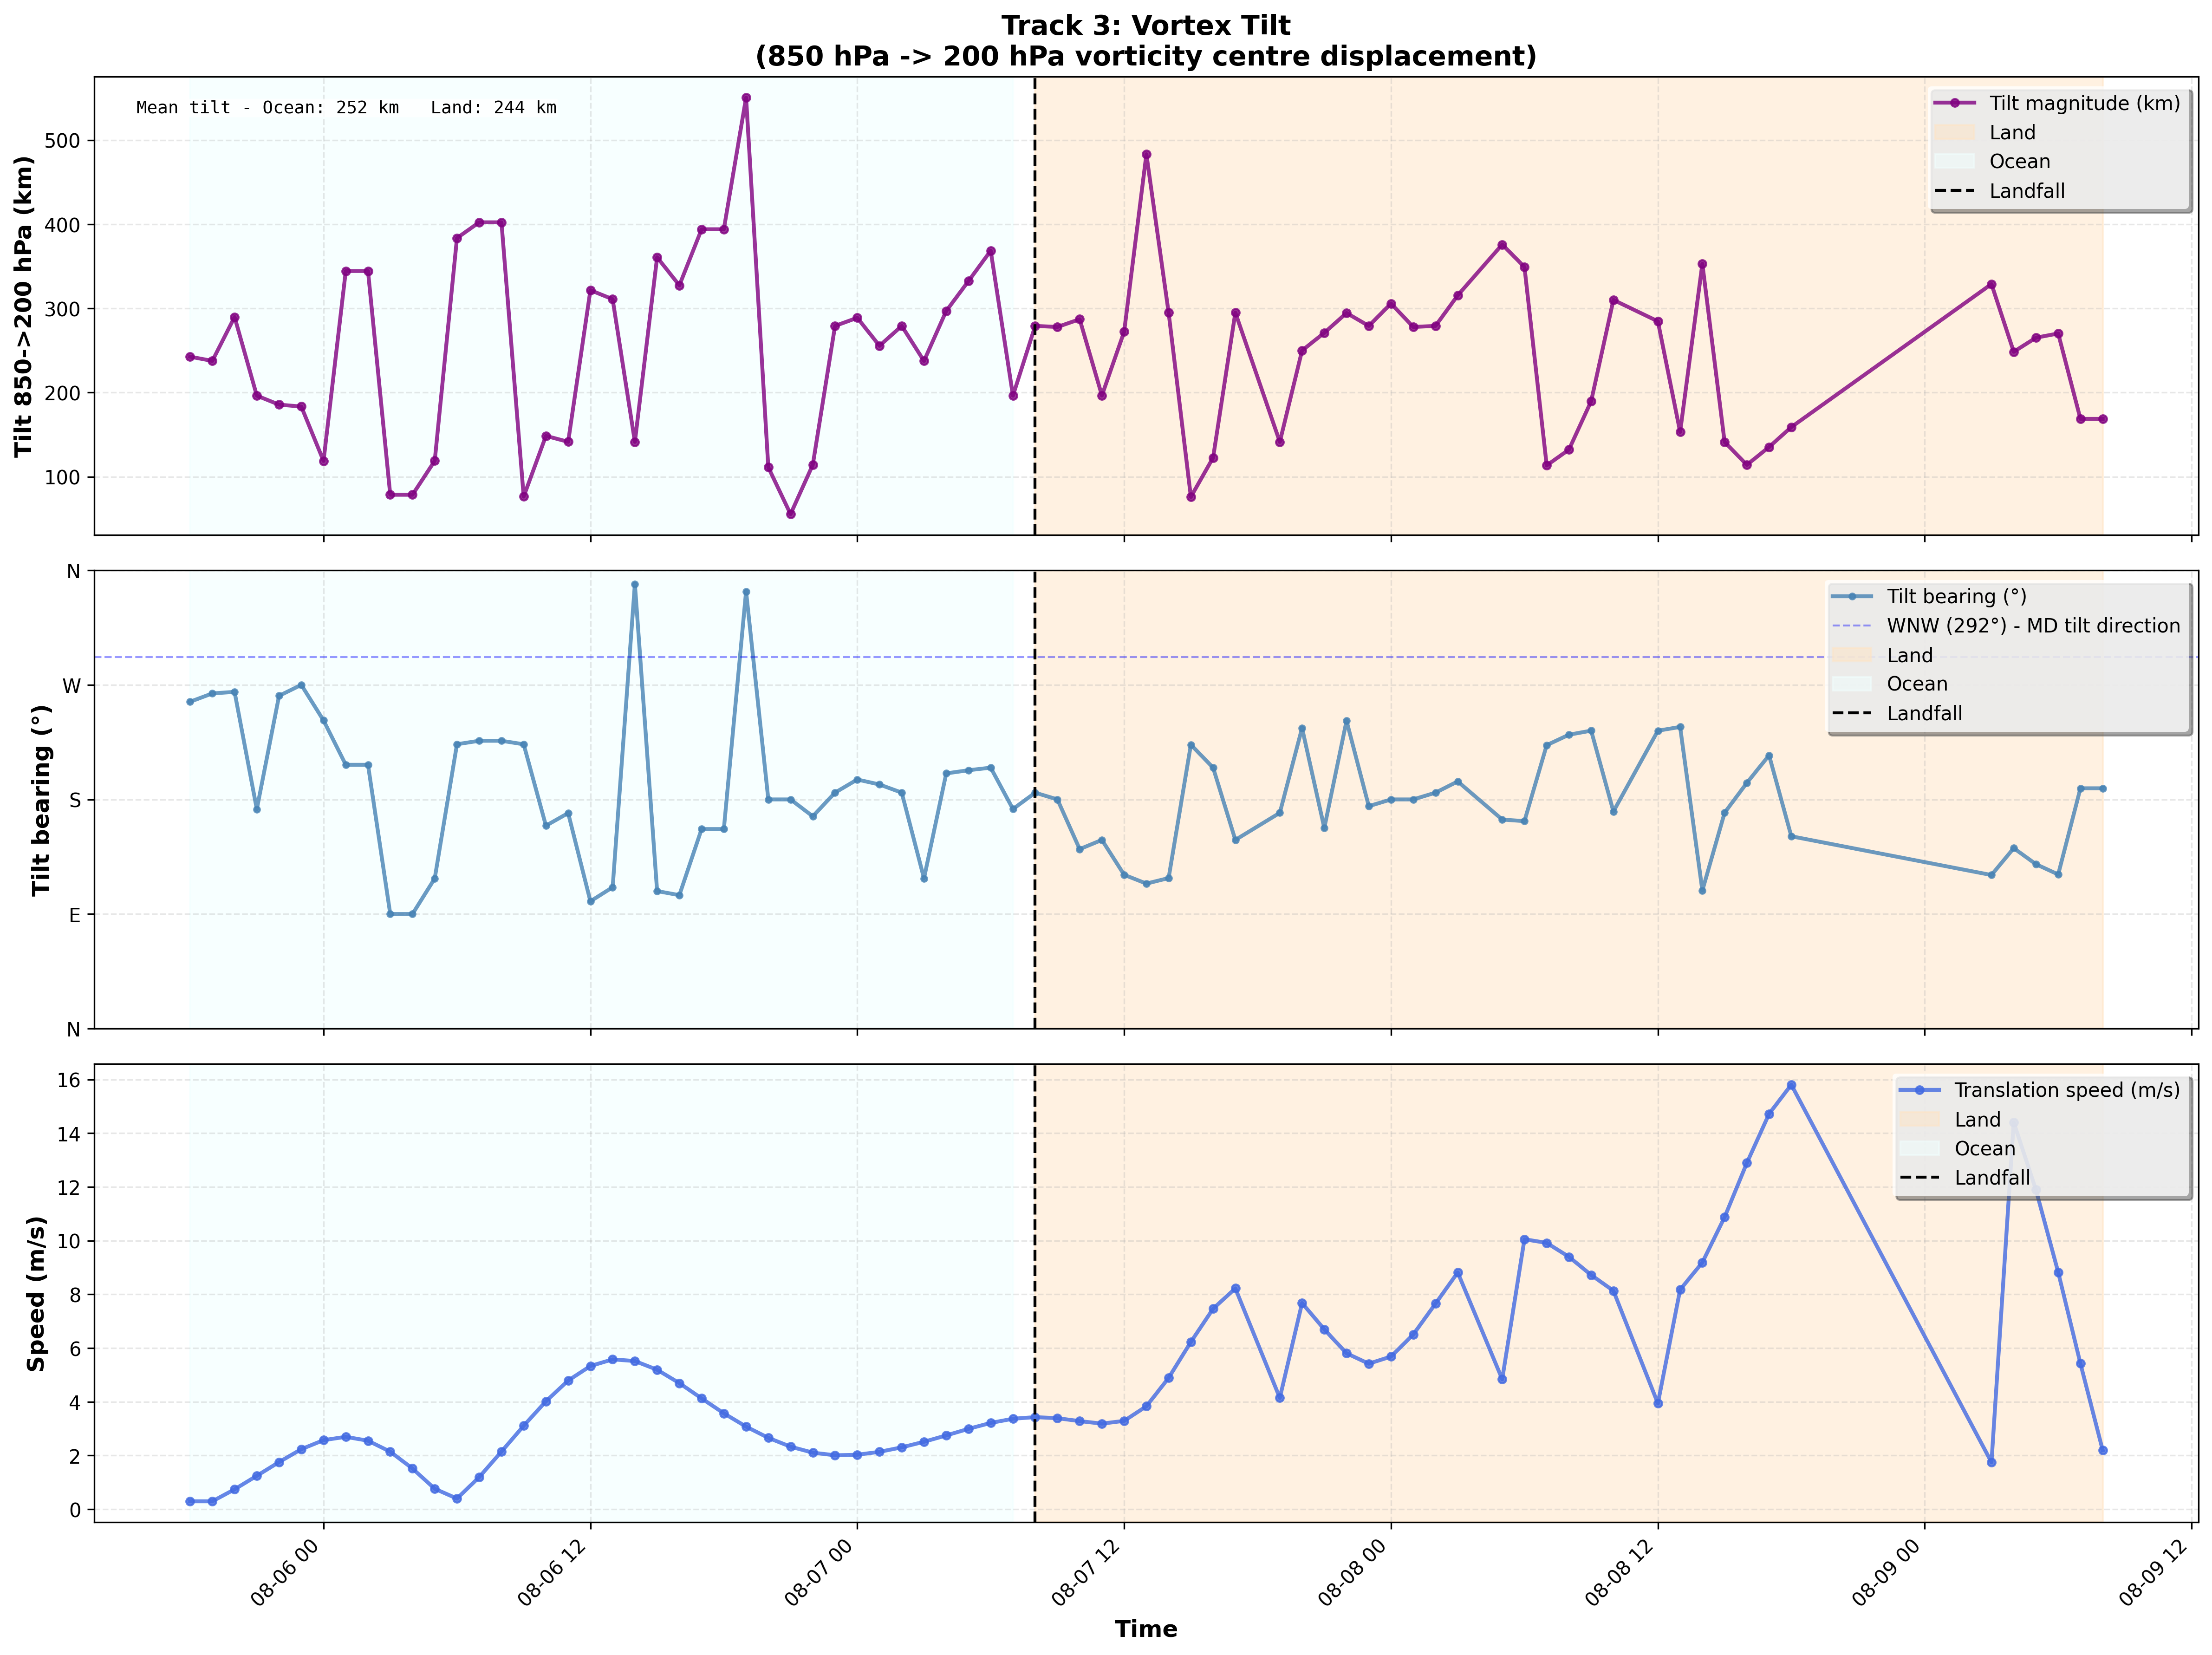
\includegraphics[width=0.95\textwidth]{Chapter2/Figs/vortex_tilt_example}
  \caption{Evolution of vortex tilt during terrain crossing,
    illustrating the structure between the low-level center and the
  upper-level warm core.}
  \label{fig:vortext_tilt}
\end{figure}

\subsection{The BOE as a Counter-Mechanism to Ghats-Induced Decay}
\label{subsec:boe_ghats_interaction}

The interaction between the Eastern Ghats blocking mechanisms
(Section~\ref{subsec:ghats_mechanisms})
and the Brown Ocean Effect is the central scientific question of this
research and its primary finding. The four decay mechanisms described
above are simultaneously counteracted by BOE surface LHF through the
following physical pathways:
\begin{enumerate}
  \item \emph{Against Mechanism 3 (moisture inflow blocking):} The
    BOE replaces the lost BoB moisture inflow with locally sourced
    evapotranspiration. While the mixing ratio of locally evaporated
    soil moisture is not identical to the warm, deep BoB moisture
    column (which extends to 500\,hPa), it is sufficient to maintain
    near-surface specific humidity and CAPE in the inner-core
    boundary layer above the BOE threshold. The key diagnostic is the
    leeward-sector dew-point depression (DPD): a BOE candidate system
    shows smaller leeward DPD increase during terrain crossing
    because surface evapotranspiration.% actively counteracts the
    % föhn-induced drying.
  \item \emph{Against Mechanism 4 (vortex tilt):} Sustained LHF at
    the land surface maintains low-level boundary-layer convergence
    (driven by the moist instability above the high-LHF zone),
    effectively keeping the surface pressure gradient alive beneath
    the stalling low-level center. This ``anchors'' the low-level
    center and limits tilt growth. A system with sustained BOE LHF
    should therefore show tilt stabilisation on the leeward side; a
    non-BOE system shows monotonically increasing tilt leading to
    structural collapse.

    Comparison of vortex tilt evolution between BOE-active and
    non-BOE systems. Figure~\ref{fig:boe_tilt_comparison} shows how
    sustained surface LHF anchors the low-level center, limiting tilt
    growth. The Figure~\ref{fig:non_boe_tilt_comparison} illustrates
    highly varying and increasing tilt leading to decoupling in the
    absence of surface moisture flux.
    \begin{figure}[H]
      \centering
      % --- BOE Stability ---
      \begin{subfigure}[b]{0.49\textwidth}
        \centering
        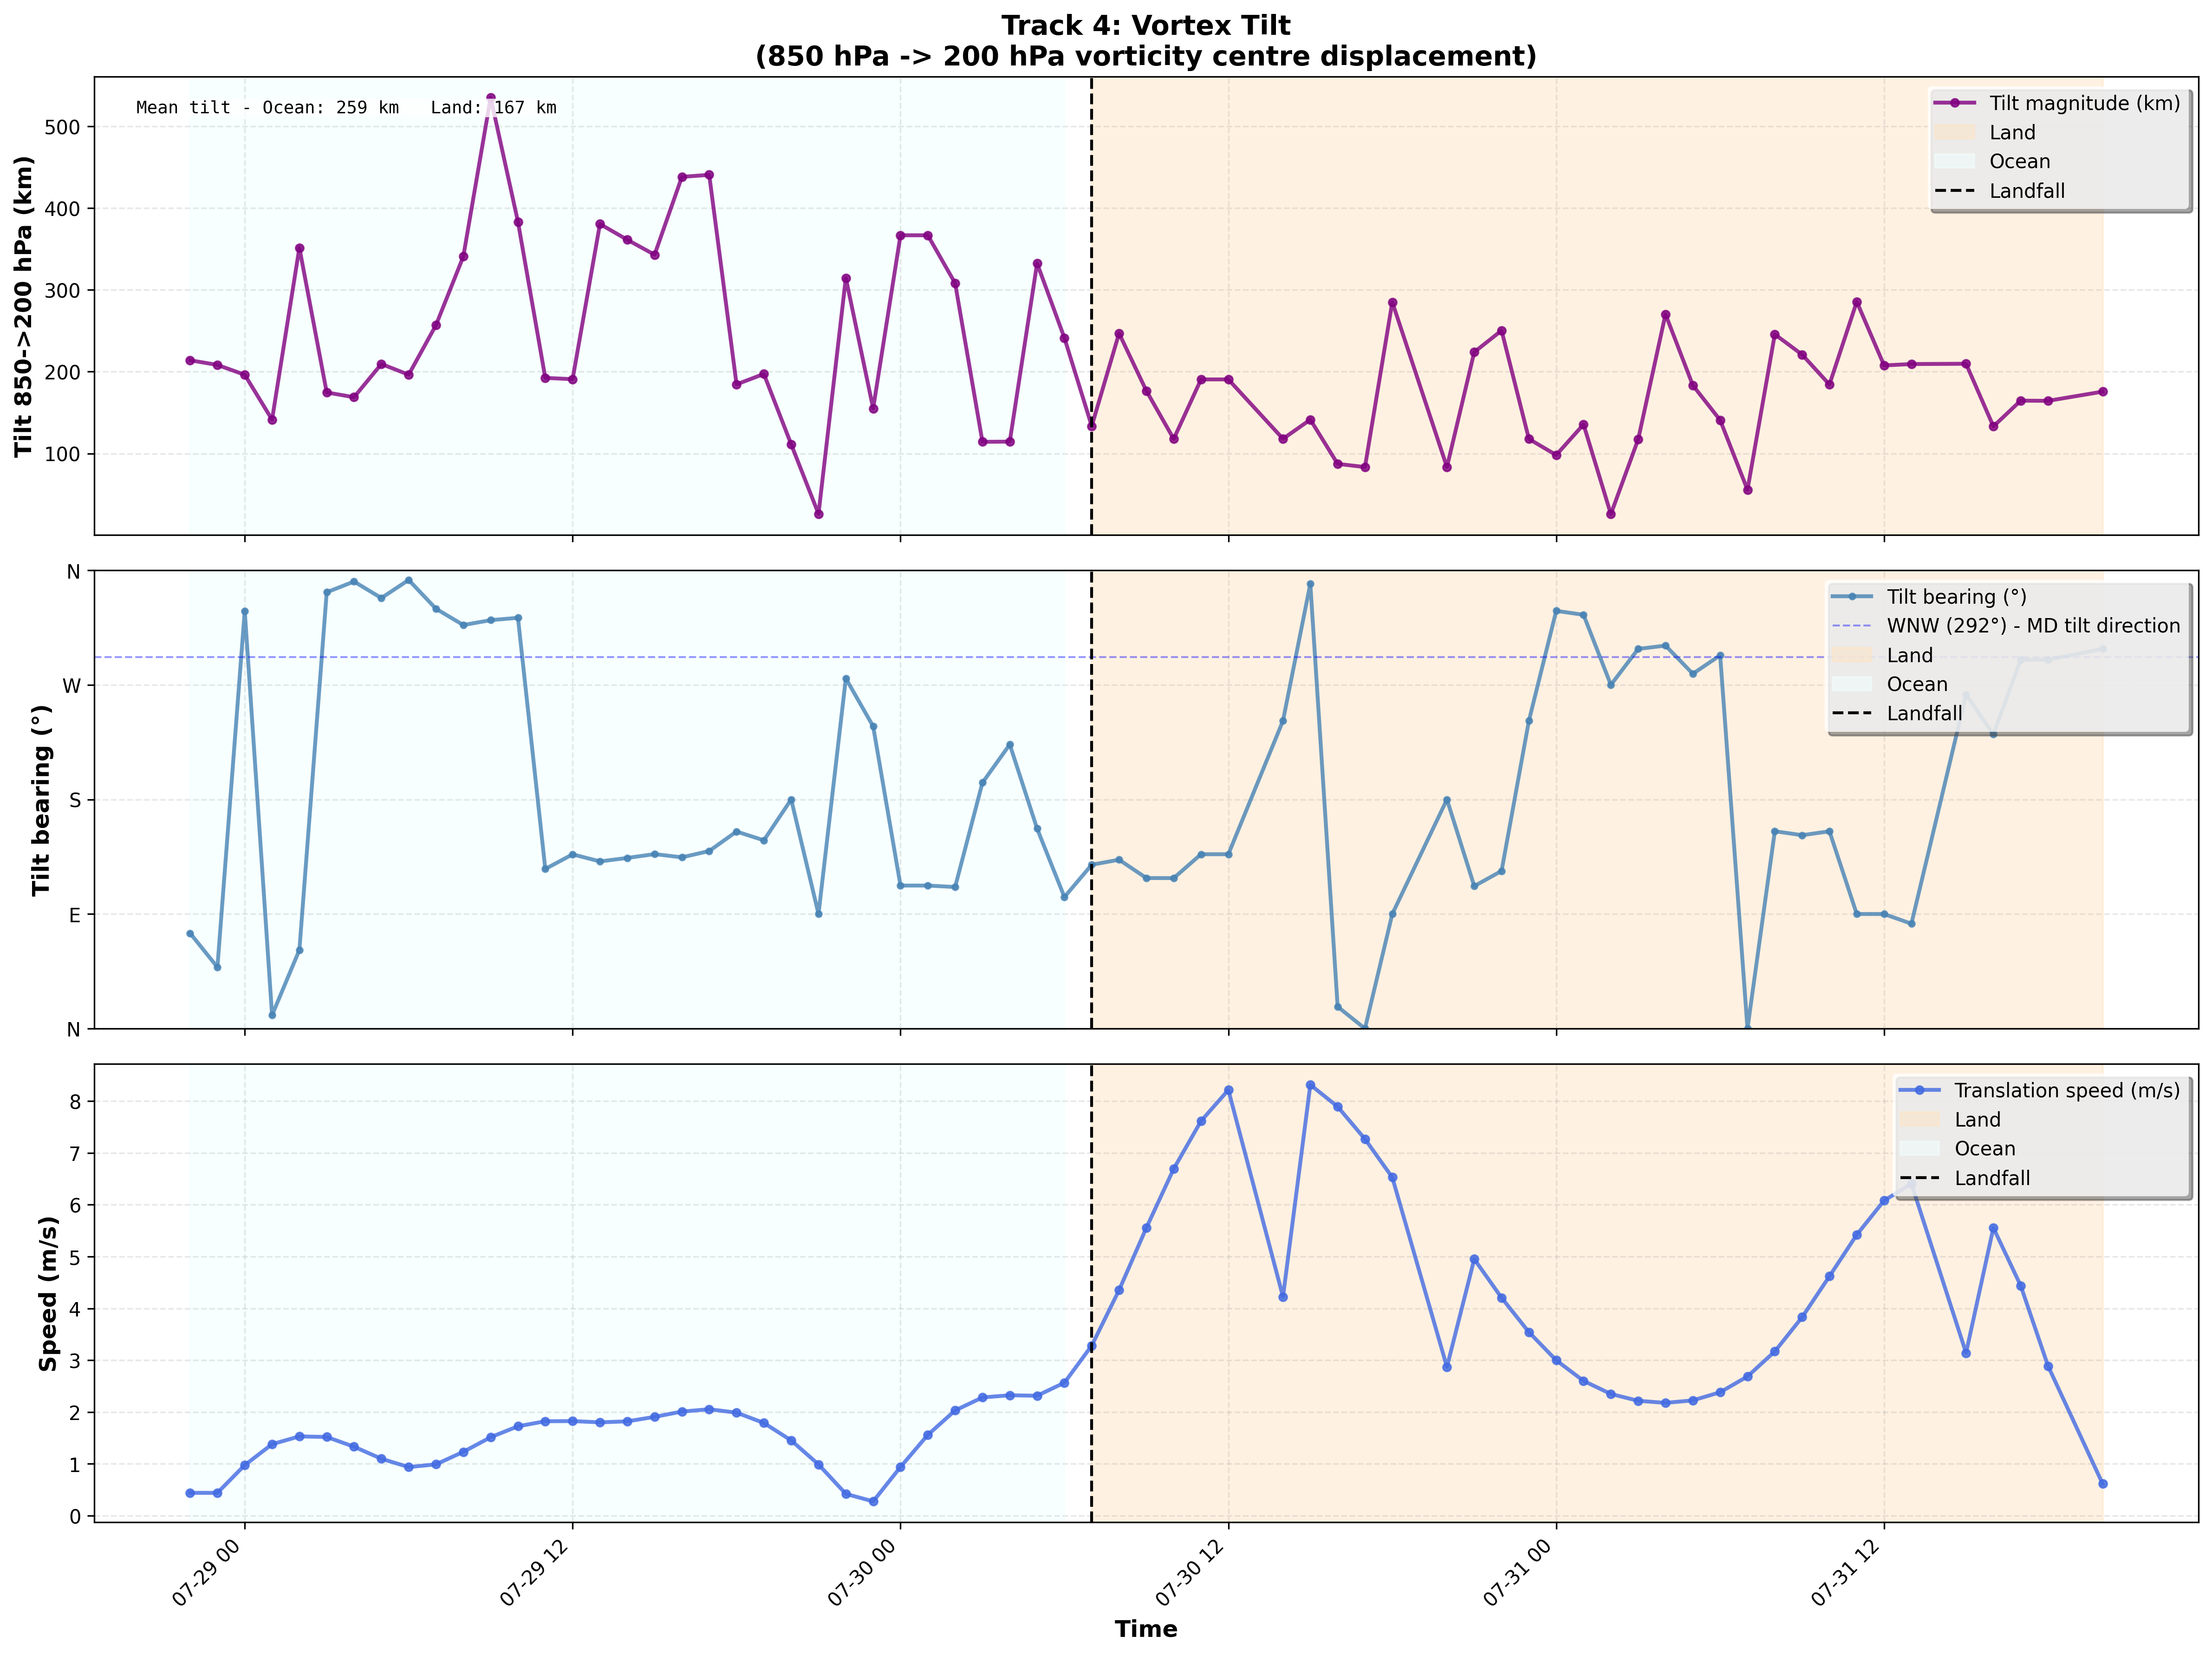
\includegraphics[width=\textwidth]{Chapter2/Figs/boe_tile_stabilisation_1.png}
      \end{subfigure}
      \hfill
      \begin{subfigure}[b]{0.49\textwidth}
        \centering
        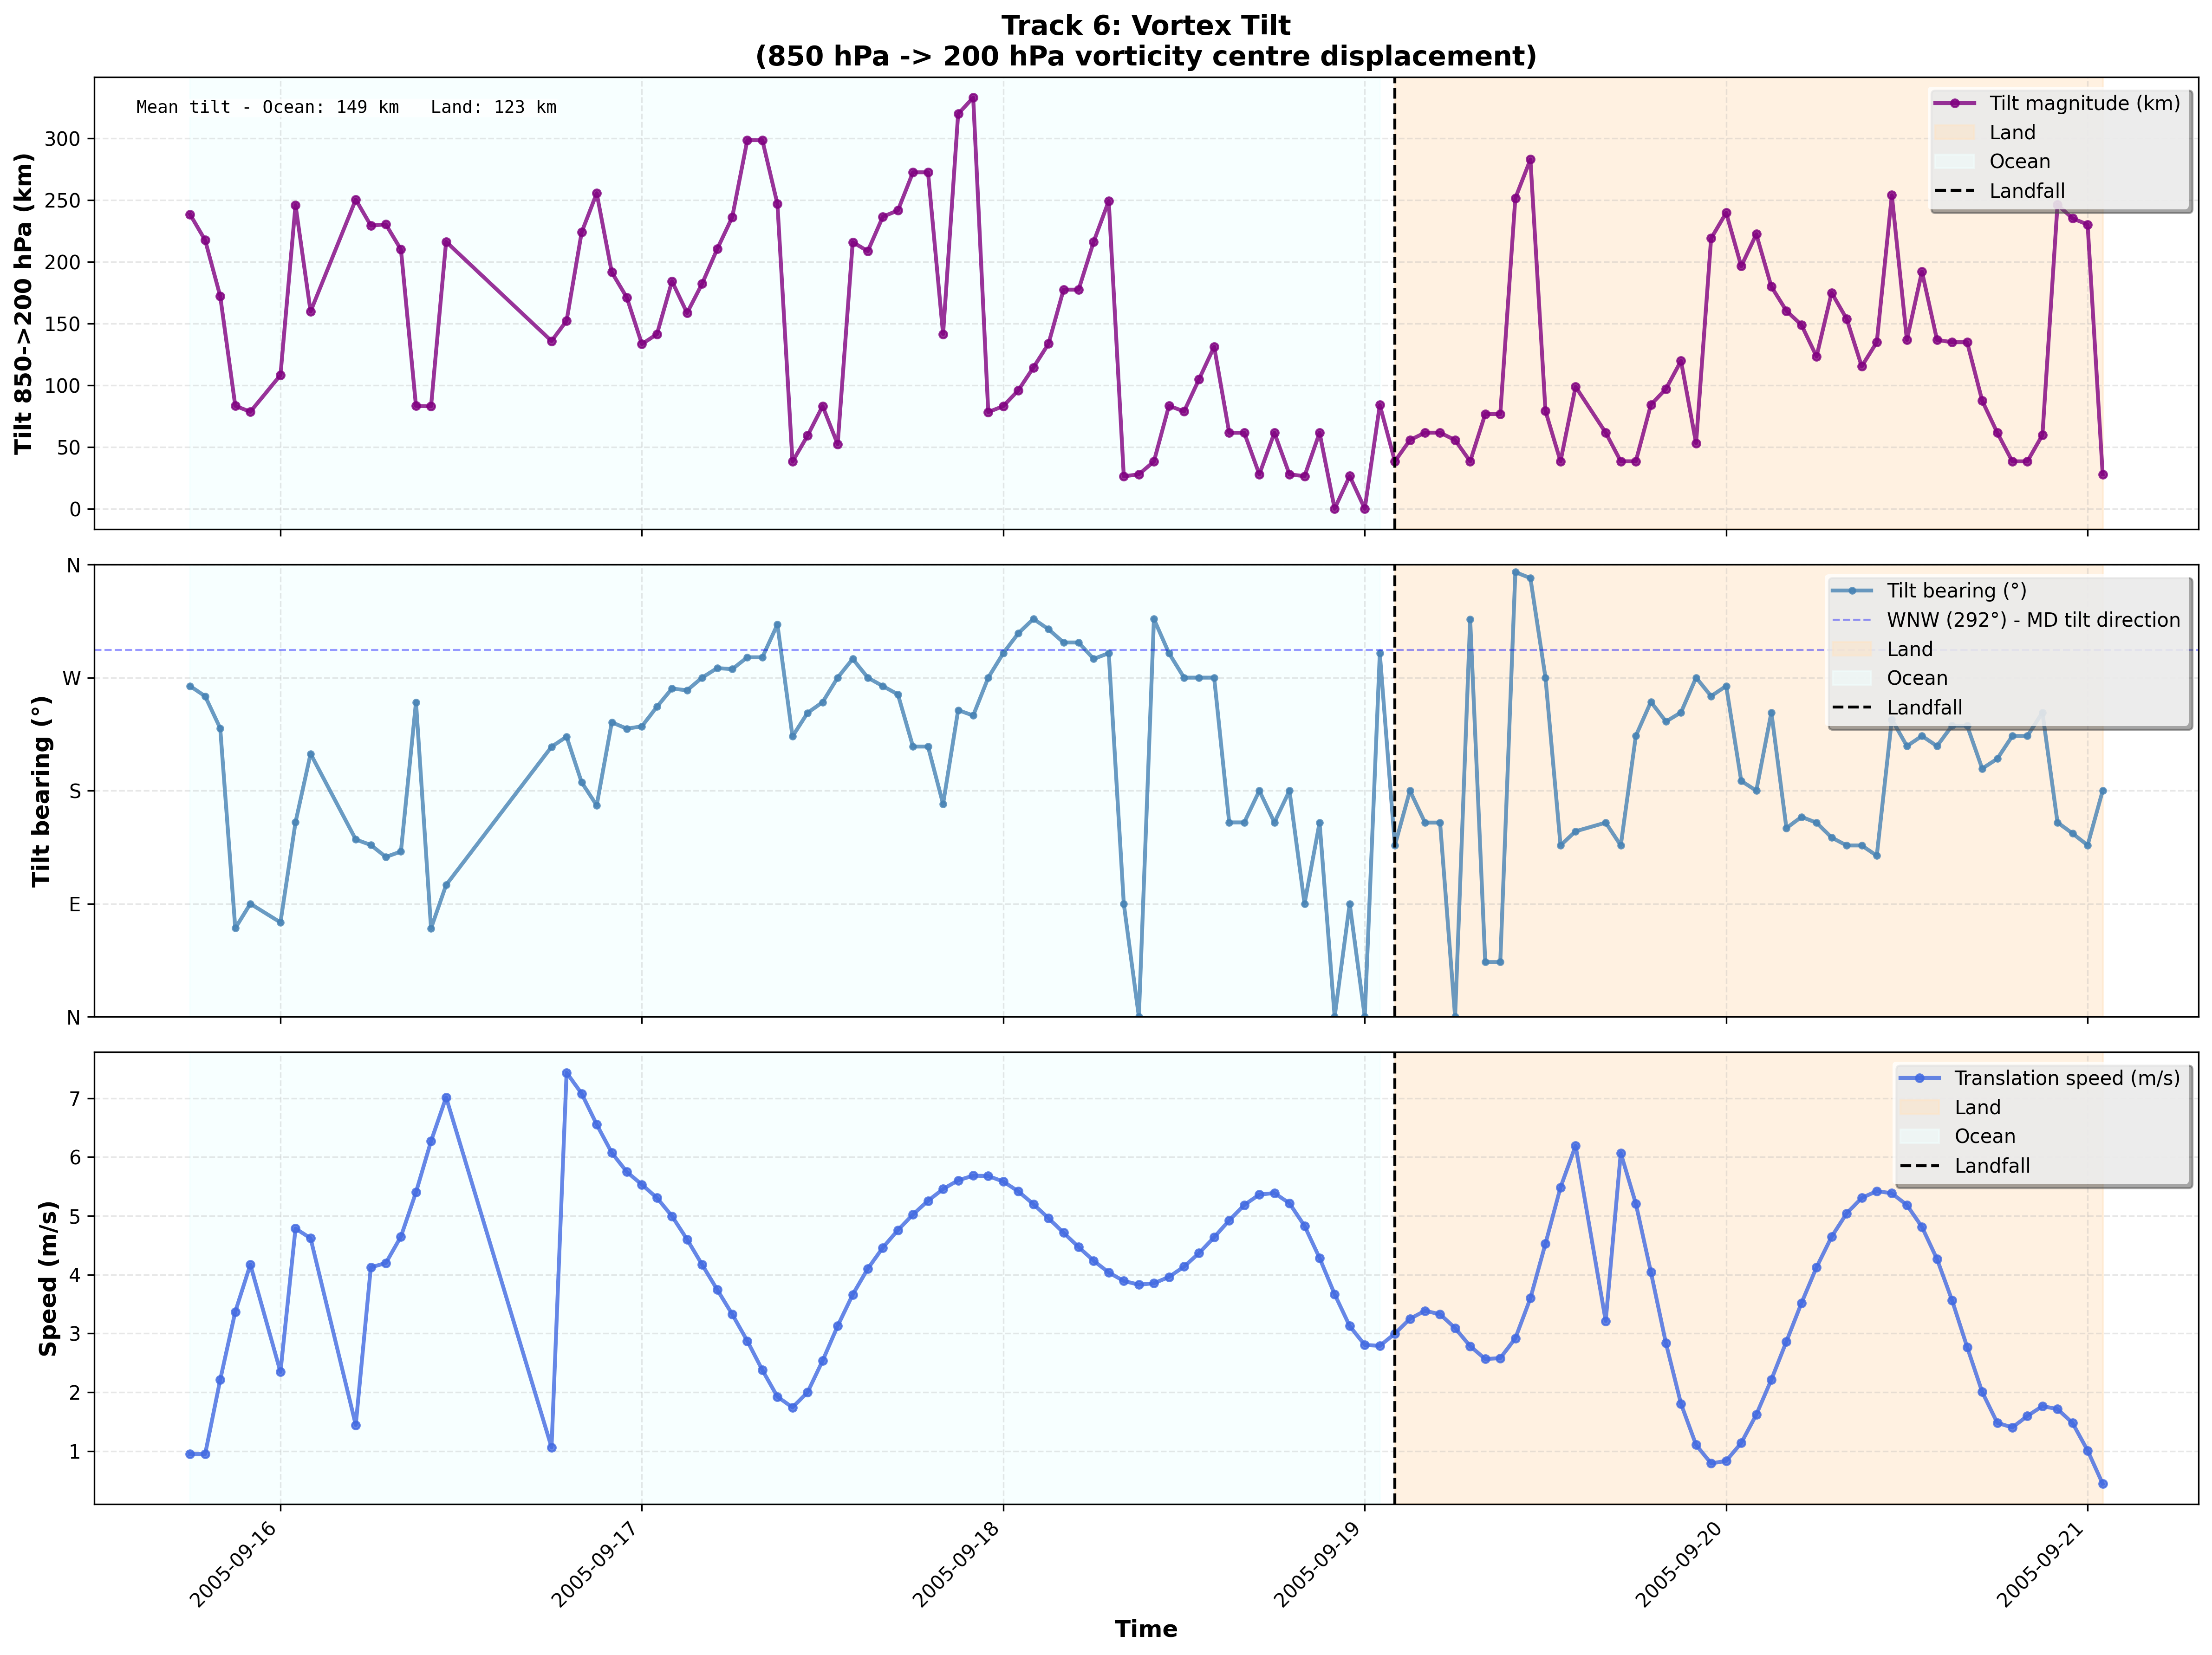
\includegraphics[width=\textwidth]{Chapter2/Figs/boe_tile_stabilisation_2.png}
      \end{subfigure}
      \caption{BOE Case: Initial crossing and Tilt stabilization}
      \label{fig:boe_tilt_comparison}
    \end{figure}
    \vspace{-0.5cm}
    \begin{figure}[H]
      % --- Non-BOE Astability ---
      \begin{subfigure}[b]{0.49\textwidth}
        \centering
        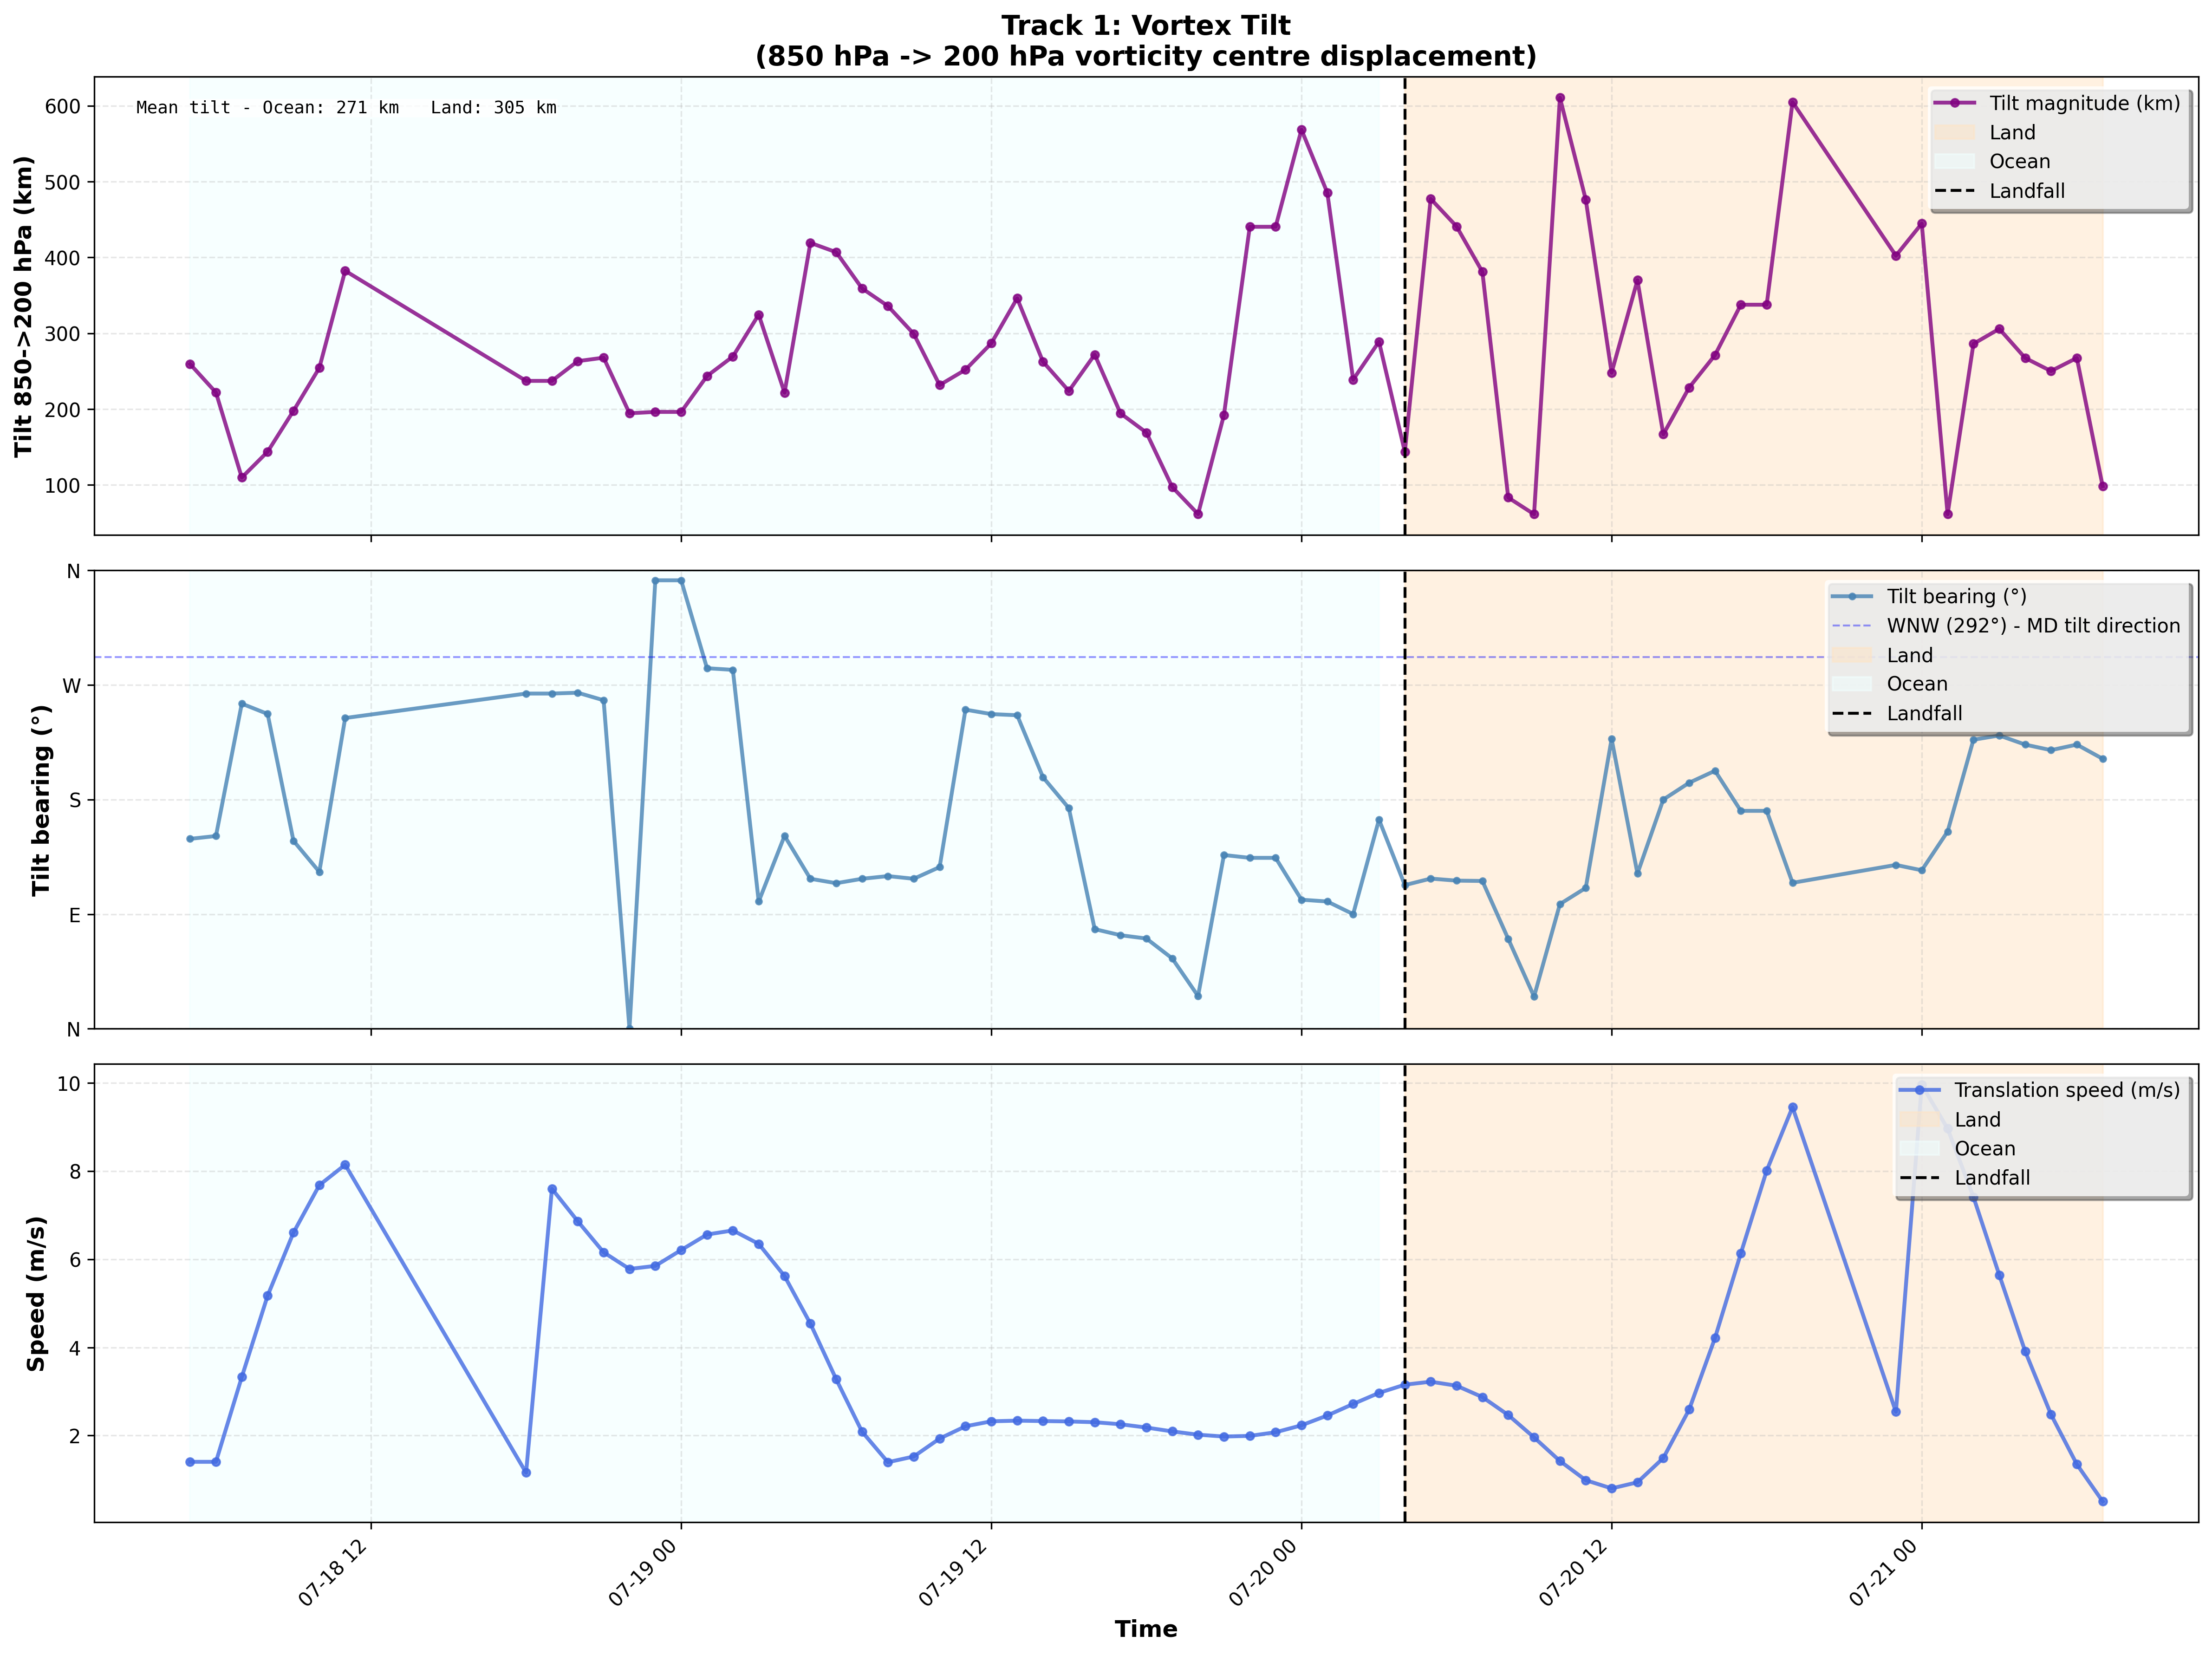
\includegraphics[width=\textwidth]{Chapter2/Figs/non_boe_tile_astabilisation_1.png}
      \end{subfigure}
      \hfill
      \begin{subfigure}[b]{0.49\textwidth}
        \centering
        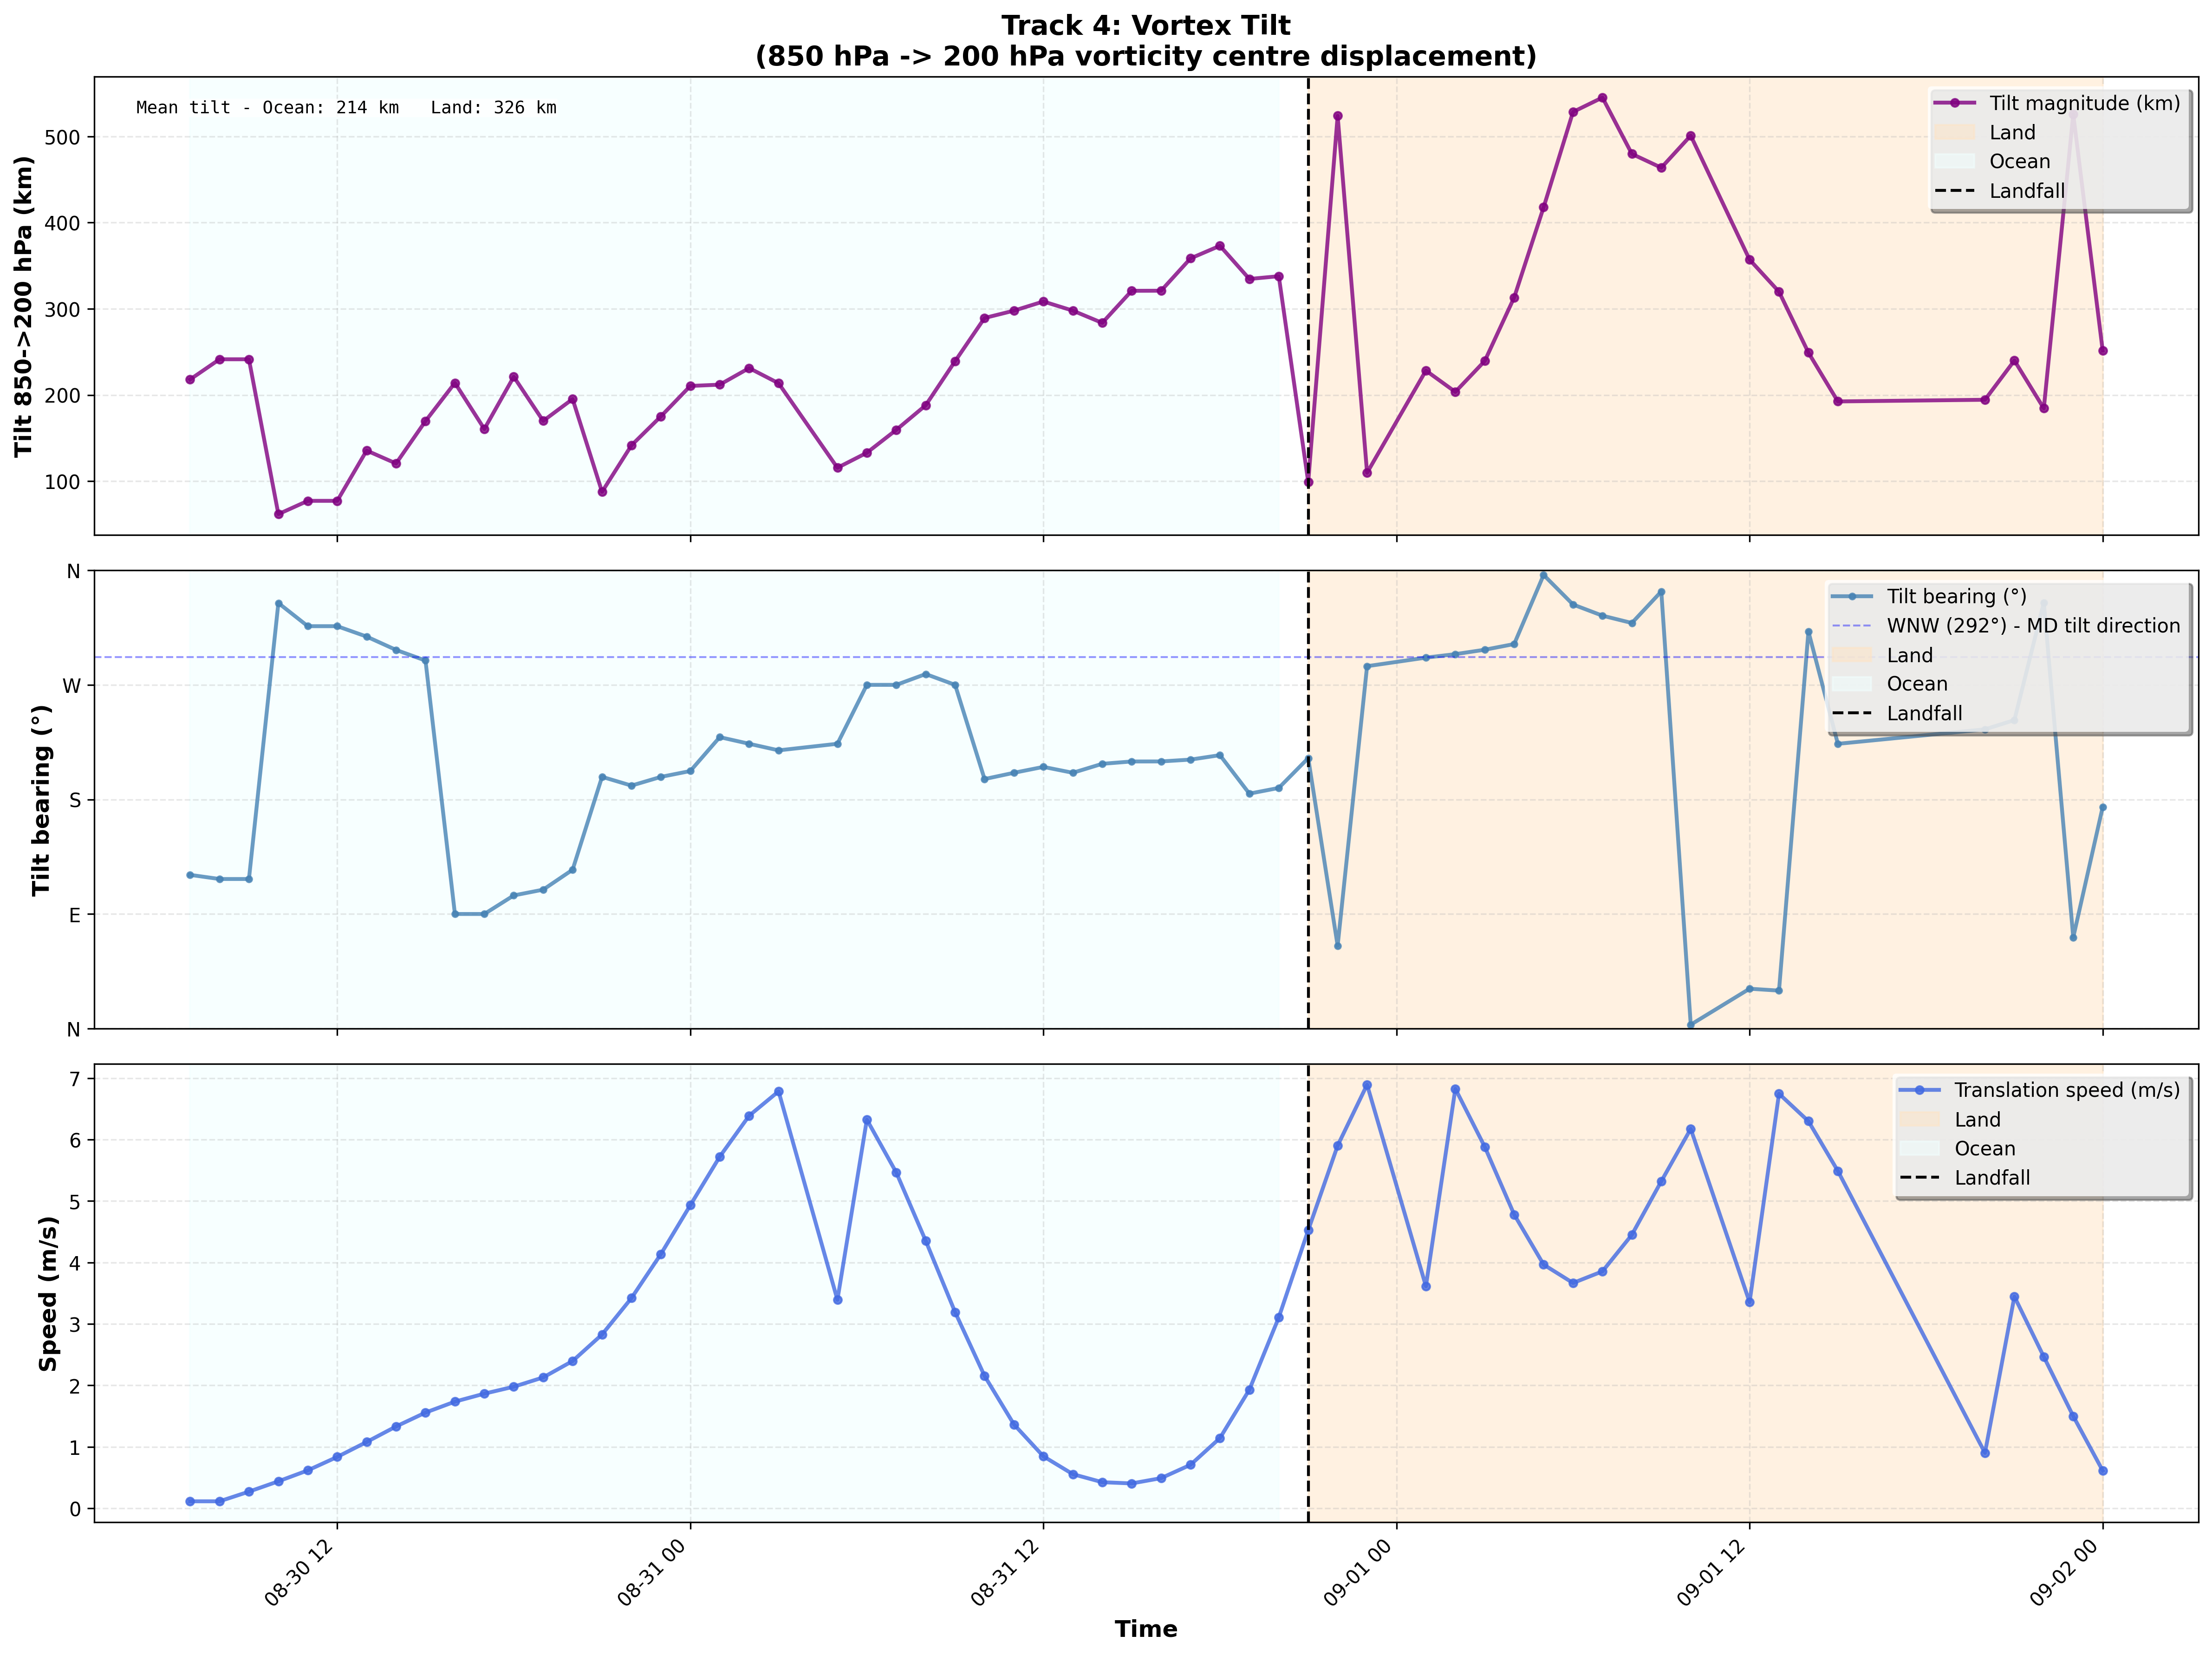
\includegraphics[width=\textwidth]{Chapter2/Figs/non_boe_tile_astabilisation_2.png}
      \end{subfigure}
      \caption{Non-BOE Case: Increasing tilt and Structural collapse}
      \label{fig:non_boe_tilt_comparison}
    \end{figure}
\end{enumerate}

The net result, confirmed by the translational speed recovery
analysis in this thesis, is that sufficiently pre-moistened surfaces
allow BOE candidates to \emph{pass through} the Eastern Ghats: they
decelerate in the terrain zone but re-accelerate on the leeward side.
This differential between BOE and non-BOE speed recovery is the
single most operationally significant finding of this study, as it
directly predicts whether a system will produce extended inland flooding.

% \yellownote{TODO: add subsection about ITCZ and it's role}
% \subsection{The Inter-Tropical Convergence Zone}
% The ITCZ marks the equatorial boundary between the northern and
% southern Hadley cells. During the NH summer it migrates to
% 5-10$^\circ$N over the Indian Ocean, providing the region of maximum
% low-level convergence into which the cross-equatorial Somali Jet
% flows. MDs forming near the BoB head are partly sustained by the
% convergent moisture flux associated with the ITCZ's northward
% migration - the same flux that the Findlater Jet intensifies and
% channels northward. The ITCZ position thus modulates both the
% moisture supply and the background vorticity available for MD genesis.
